%% LyX 2.0.7.1 created this file.  For more info, see http://www.lyx.org/.
%% Do not edit unless you really know what you are doing.
\documentclass[12pt,oneside,english]{amsbook}
\usepackage{mathptmx}
\renewcommand{\familydefault}{\rmdefault}
\usepackage[T1]{fontenc}
\usepackage[utf8]{luainputenc}
\usepackage{geometry}
\geometry{verbose,tmargin=1.25in,bmargin=1.25in,lmargin=1.25in,rmargin=0.75in}
\usepackage{float}
\usepackage{amsthm}
\usepackage{amstext}
\usepackage{graphicx}
\usepackage{setspace}
\usepackage[numbers]{natbib}
\usepackage{subscript}
\doublespacing

\makeatletter

%%%%%%%%%%%%%%%%%%%%%%%%%%%%%% LyX specific LaTeX commands.
\newcommand{\lyxmathsym}[1]{\ifmmode\begingroup\def\b@ld{bold}
  \text{\ifx\math@version\b@ld\bfseries\fi#1}\endgroup\else#1\fi}

%% Because html converters don't know tabularnewline
\providecommand{\tabularnewline}{\\}

%%%%%%%%%%%%%%%%%%%%%%%%%%%%%% Textclass specific LaTeX commands.
\numberwithin{section}{chapter}
\numberwithin{equation}{section}
\numberwithin{figure}{section}
\theoremstyle{plain}
\newtheorem{thm}{\protect\theoremname}

%%%%%%%%%%%%%%%%%%%%%%%%%%%%%% User specified LaTeX commands.
\usepackage{titlesec}
\usepackage{amsmath}
\usepackage{graphicx}
%\usepackage{epsfig}
\usepackage{epic}
\usepackage{eepic}
\usepackage{eepicemu}
\titlespacing*{\chapter}{0pt}{0.45in}{20pt}
\titleformat{\chapter}[display]
{\normalfont\bfseries\normalsize\centering}{\MakeUppercase{\chaptertitlename}\ \thechapter}{0pt}{\normalsize\bfseries\MakeUppercase}
\titleformat{\section}
  {\normalfont\normalsize\MakeUppercase}
  {\thesection}{1em}{}
\titleformat{\subsection}
  {\normalfont\normalsize}
  {\thesubsection}{1em}{}
\newcommand{\taba}{\hspace*{2em}}
\newcommand{\tabb}{\hspace*{4em}}
\newcommand{\tabc}{\hspace*{6em}}
\renewcommand{\arraystretch}{2.0}

\makeatother

\usepackage{babel}
\providecommand{\theoremname}{Theorem}

\begin{document}
\tableofcontents{\makeatletter
\let\toc@pre\relax
\let\toc@post\relax
\makeatother}

\begin{center}
\textbf{AN APPROXIMATION TO RATE-EQUALIZATION FAIRNESS WITH LOGARITHMIC
COMPLEXITY}
\par\end{center}

\begin{center}
Suparn Gupta, Masters
\par\end{center}

\begin{center}
The University of Texas at Dallas, 2014\linebreak{}
\linebreak{}

\par\end{center}

\begin{center}
Supervising Professor: Jorge Arturo Cobb\linebreak{}
\linebreak{}

\par\end{center}


\section*{\centerline{\textbf{ Abstract}}}

\noindent Scheduling protocols that provide both rate and fairness
guarantees, such as Weighted Fair Queuing (WFQ) distributes the unused
bandwith among flows in proportion to their reserved rate. Flows with
higher reservation rate thus receive a larger share of bandwith than
those with lesser reserved rates.

\noindent In an earlier work \citep{Cobb-REQ}, a new approach to
allocate unused bandwidth known as rate-equalization (REQ) was proposed,
in which the unused bandwidth is first given to the flows with least
reserved rates. However, this algorithm has a per-packet complexity
of \emph{O(n)} where \emph{n} is the number of flows.

\noindent The present study proposes a new algorithm, which is an
approximation of REQ fairness with logarithmic per-packet complexity.
The simulation results endorse than in different practical scenarios,
the behavior of the new algorithm is quite similar to that of pure
REQ fairness.




\chapter{Introduction}

\noindent \begin{flushleft}
In a network of various interconnected nodes which provides QoS, a
certain amount of bandwidth is reserved for each flow. A scheduling
protocol is implemented to make decisions about the packet transmission
from each backlogged flow. Selection of such protocol is a crucial
decision because of the complexity and execution cost. Any such scheduling
protocol can be analyzed on the basis of different kinds of guarantees
it provides. Two such metrics of analysis are rate and fairness guarantees.
\par\end{flushleft}


\subsubsection*{Rate Guarantee:}

A flow requests for a certain amount of bandwidth (rate) in the network
before it begins transmitting packets. If the network has enough bandwidth
available, it grants the reservation request. Otherwise, the request
is denied. A scheduling protocol which provides rate guarantee assures
that a flow gets atleast its reserved bandwidth at all times while
it is active. A flow may receive more bandwidth than what it originally
requested for, if bandwidth gets available. Such a guarantee thus
ensures that any flow gets atleast a certain amount of service in
the scheduler.


\subsubsection*{Fairness:}

If the network is not congested, it might be possible that a part
of bandwidth is unused. It may happen for two reasons:
\begin{enumerate}
\item There is some unallocated bandwidth available in the network.
\item A set of flows are not fully utilizing their share of allocated bandwidth
by transmitting packets at a slower rate than their service rate.
\end{enumerate}
To use the resources efficiently, a scheduler thus distributes the
unused bandwidth among the flows fairly while maintaining firewalls
between them so that the allocation is followed strictly by all the
flows. Fairness means a flow should not be “punished” (temporarily
denied service) if it exceeds its reserved rate to take advantage
of unused bandwidth in the channel. The way in which each protocol
distributes the unused bandwidth is different. 

If a flow gets empty, the scheduler starts serving the packets from
the next non empty flow. Such a scheduler will be work-conserving
since it doesn't let resources go to waste. In certain scenarios,
a scheduler may decide not to distribute the unused bandwidth. Such
a scheduler is non-work conserving. In the next few sections, a number
of well known scheduling protocols are described.


\section{Scheduling Protocols}

Real-time applications, such as interactive audio and video, require
from the network an assurance that their packets will be forwarded
with a lower bound on the forwarding rate and also with a bounded
end-to-end delay. Rate-guaranteed schedulers \citep{Cobb-Flow-Theory-ToN},
\citep{leaveintime}, \citep{NOSSDAV-95-Vin} is a family of protocols
that is able to provide this assurance. Iconic examples of this protocol
family include Virtual Clock (VC) \citep{VC-Lam}, \citep{VC-Lixia}
and Weighted Fair Queuing (WFQ) \citep{GPS-Parekh}, plus their many
variations. One desirable property of a rate-guaranteed scheduler
is fairness. Some protocols, such as Virtual Clock, are unfair, while
others, like WFQ, are fair. Being able to provide fairness is desirable
for some applications whose can adapt to changes in the bandwidth
provided by the network. Examples of such flows are file transfers
and multi-resolution video \citep{hopbyhop}. The sources of these
flows will likely reserve from the network the smallest packet rate
necessary to receive a minimum quality of service. The source is then
able to detect that additional bandwidth is available due to side-effects
observed in the network, such as a smaller end-to-end delay, and increase
its packet-generation rate accordingly. Speaking generally of scheduling
protocols, rate guarantee and fairness can be considered as two extreme
ends between which various rate guaranteed scheduling algorithms fit
in. 

Prior to begining the discussion about scheduling protocols, it is
important to establish a formal notion of a flow. A flow :
\begin{enumerate}
\item is a stream of packets where each packet follows the same path in
the network.
\item avails a certain minimum amount of service in the network.
\end{enumerate}
Each packet is uniquely bound to a particular flow which can be identified
by analysing the headers in the packet. At any given time \emph{t},
if a flow has packets in its queue, it is known as a \emph{backlogged}
flow. Otherwise, a flow with empty queue at any given time t is \emph{idle}.
Consider a set of all the flows represented by \emph{W}. Then at any
given time \emph{t}, the set of backlogged flows given by \emph{B}
satisfies \emph{$B \subseteq\ W$.}

In the following sections, consider an output channel with a capacity
\emph{C} and a set of flows \emph{W} in the fluid server such that
each flow is represented by \emph{f\textsubscript{\emph{i }}}$\mathcal{\epsilon}$\emph{
W, where $1\leq i\leq n$. }Let \emph{B }represent the set of backlogged
flows in the fluid server.


\subsection{Weighted Fair Queuing (WFQ)}

A Generalized Processor Sharing (GPS) discipline provides rate and
fairness guarantees. However, since it models a fluid server, it assumes
that the scheduler can serve all the flows. However, a real scehduler
has to transmit a packet from one flow at any given time and thus,
it is impossible to practically realize a GPS system. Several packetized
approximations which follow the footsteps of GPS have been proposed
in past many years. Out of such known algorithms, Weighted Fair Queuing
is well known to provide both rate and fairness guarantees\emph{.}
It assures that \emph{(a)} each flow gets atleast the amount of bandwidth
it reserved and \emph{(b)} the unused bandwith is allocated among
the flows in proportion of their reserved rates. Thus the flows with
higher reserved rates get the larger share of unused bandwidth than
those with smaller reserved rates. 

Each flow \emph{$f_{i}\;\epsilon\; B$} is assigned a weight \emph{w\textsubscript{\emph{i}}
}and gets the bandwidth \emph{$c_{i}$} allocated as per the following
rule:

\begin{equation}
c_{i}=\frac{w_{i}}{\sum_{x}w_{x}},\;\;\;\; f_{x}\;\epsilon\; B
\end{equation}


\newpage{}There are two schedulers (servers) in the system:
\begin{enumerate}
\item Fake or bit-by-bit scheduler, which forwards a few bits of each flow
at a time (i.e. fractions of a packet)
\item Real scheduler, which

\begin{itemize}
\item assigns timestamps to packets.
\item sends out packets in non-decreasing order of timestamp.
\end{itemize}
\end{enumerate}
The timestamp is the “virtual” finishing time of the packet at the
fake server. The virtual time \emph{V(t)} at real time t is the “bit
number” or “round-number” in the fake bit-by-bit server at real time
\emph{t}. In case of fair queuing, \emph{V(t)} is increased by 1 every
time one bit is forwarded from all the flows in the fake server. In
case of WFQ, \emph{V(t)} is increased by 1 every time when for each
flow $f_{i}\;\epsilon\; B$, $w_{i}$ bits are forwarded from all
the flows in the fake server. If there are fewer number of flows in
the server, the \emph{virtual time} will run faster. Also, for each
tick in \emph{virtual }time, the number of bits forwarded for flows
with higher weights is more than those with lower weights. 

Let $F_{f,i}$ be the virtual time when the \emph{i-th} packet of
flow \emph{f} exits the bit-by-bit server, $A_{f,i}$ be the virtual
time when the \emph{i-th} packet of flow \emph{f} exits the bit-by-bit
server. Then following relation can be established.

\begin{equation}
F_{f,i}=max(V(A_{f,i}),\; F_{f,i-1})+\frac{L_{f,i}}{w_{f}}
\end{equation}


\begin{center}
where $L_{f,i}$ is the length of \emph{i-th} packet of flow f
\par\end{center}

In \citep{GPS-Parekh}, it has been proven that if the rate admission
control is maintained using the leaky bucket, end to end delay guarantee
can be achieved. A packet gets out of the real server by the time
it gets out of the fake server plus a constant. Thus,

\begin{equation}
Finishing\; time=F_{f,i}+\frac{L_{max}}{C}\label{eq:exit-bound-wfq}
\end{equation}


\begin{center}
where $L_{max}$ is the maximum length of the packet.
\par\end{center}

It was long known that the WFQ can be implemented with a per-packet
complexity of \emph{O(n)}, until Valente \citep{WFQlogN} proposed
a way to implement WFQ in \emph{O(log(n))} per-packet complexity.
He uses a complex scheme to organize the breaking points in a search
tree to optimize searches. 


\subsection{Worst-case Fair Weighted Fair Queueing (WF\textsuperscript{2}Q)}

In \citep{GPS-Parekh}, Parekh stated a number of relationships between
a GPS and a packetized approximation of GPS, which he called as PGPS
(identical to WFQ). Two main claims were as follows:
\begin{enumerate}
\item A packet gets out of a PGPS scheduler no later than it gets out of
GPS scheduler with a delay of atmost one packet transmission time.
\item PGPS cannot lag behind the GPS scheduler by more than one packet transmission.
\end{enumerate}
From above two claims, one may deduce that a PGPS scheduler offers
a service which is almost identical to a GPS scheduler with a variation
of atmost one packet transmission time, which was once a popular belief
until Bennet et al.\citep{Hui-WF2Q} proved that there can be significant
discrepances between a PGPS and a GPS scheduler. They claim that the
PGPS scheduler can be far ahead of GPS in terms of service given to
a session leading to an unfair behavior of the protocol towards other
sessions.

In PGPS or WFQ approximation of GPS, packets are transmitted according
to the order of their timestamps. It might happen that a packet may
get transmitted in the PGPS before it exits the GPS scheduler. In
this case, the next packet of the session might start receiving service
even before the first packet finishes in GPS. This may lead WFQ to
run ahead of GPS thus favoring a particular flow. In \citep{Hui-WF2Q},
a modified policy for selecting packets for transmission has been
proposed which is called WF\textsuperscript{2}Q. According to this
policy, when a WFQ scheduler selects the next packet for transmission,
it choses a packet among those, which have already started receiving
service in corresponding GPS system. Also, it has been established
that with WF\textsuperscript{2}Q policy, the system offers service
almost identical to GPS with a maximum difference of one packet transmission.
Also, WF\textsuperscript{2}Q scheduler is proven to be work conserving.


\subsection{Virtual Clock (VC)}

Another packet service discipline has been proposed in by Zhang \citep{VC-Lixia}
which is known as Virtual Clock algorithm. The basic concept of this
algorithm is somewhat similar to Time Division Multiplexing (TDM),
which maintains a perfect firewall among various sessions. In TDM,
each session can transmit data only in a particular time slot. However,
this turns out to be inefficient on resource utilization as a time
slot may get wasted if the session doesn't have any packet to transmit.
Virtual Clock preserves the firewall property of a TDM and ensures
work conserving nature of the scheduler. 

In VC algorithm, two clocks are implemented, a real clock and a virtual
clock. Whenever, a packet is received at the queuing node, it is timestamped
with a virtual clock value. The packets are served in non-decreasing
order of virtual clock timestamps of each packet. Suppose that a session
\emph{f} has a reserved bandwidth of $R_{f}$. Then for each such
flow a value known as $Vtick_{f}$ \citep{VC-Lixia}is calculated
according to the following relationship:

\begin{equation}
Vtick_{f}=\frac{1}{R_{f}}\label{eq:1.1.4}
\end{equation}


Now consider the \emph{i-th} packet of flow \emph{f} represented by
$p_{f,i}$. Using \ref{eq:1.1.4}, the Virtual Clock value $VC_{f,i}$
for $p_{f,i}$ can be calculated using the following equation:

\begin{equation}
VC_{f,i}=VC_{f,i-1}+Vtick_{f}
\end{equation}


One important point to note here is that, flows which generate packets
at a slower rate may accumulate credits over the time and thus create
unfairness in the system towards other flows. This is taken care of
by periodically synchronizing the Virtual Clock values with the real
time so that VC values don't fall far behind of real time. In\citep{VC-Lam},
it has been proven that Virtual Clock Algorithm has delay bound which
is identical to that of WFQ. However, VC is not a fair scheduling
policy. Flows which transmit data at a speed higher than their reserved
rates may get extra bandwidth for sometime if its available. But in
later time, since their VC values will be far ahead of slower flows,
they will get punished. This behavior has been modified in a scheme
proposed in \citep{leapforward}. This scheme gives an end-to-end
delay guarantee similar to WFQ and also exhibits throughput fairness.


\chapter{QoS Model}

In all the previously discussed algorithms, the rate guarantee is
always ensured by providing atleast the reserved rate of service to
a session. The way fairness is ensured varies with different protocols.
Algorithms, which follow the GPS discipline exhibit fairness by distributing
the unused bandwidth in proportion to the reserved rates of flows.
Algorithms like Leap Forward Virtual Clock \citep{leapforward} maintain
fairness by moving misbehaved sessions to a separate queue while keeping
the well-behaved flows together. 

The QoS model presented here is based on the models of \citep{Cobb-Flow-Theory-ToN}
and \citep{leaveintime}. A \emph{network }is a set of computers connected
via point-to-point communication channels. A flow\emph{ }is a sequence
of packets, all of which originate at the same source computer and
are destined to the same computer. All packets of a flow must traverse
the network along a fixed path.

Each flow is characterized by its data rate and an upper bound on
its end-to-end delay. Before a source introduces a new flow to the
network, enough network resources are reserved to ensure the flow's
delay bound is not violated. If enough resources are not available,
the flow is rejected.

Each output channel of a computer is equipped with a packet scheduler
(see Figure \ref{fig:fig1}). A scheduler receives packets from flows
whose path traverses its output channel. Whenever its output channel
becomes idle, the scheduler chooses a received packet and forwards
it over the output channel. A packet\emph{ exits} a scheduler when
its last bit packet is transmitted by the output channel. 

\newpage{}

\begin{figure}[tb]
\centering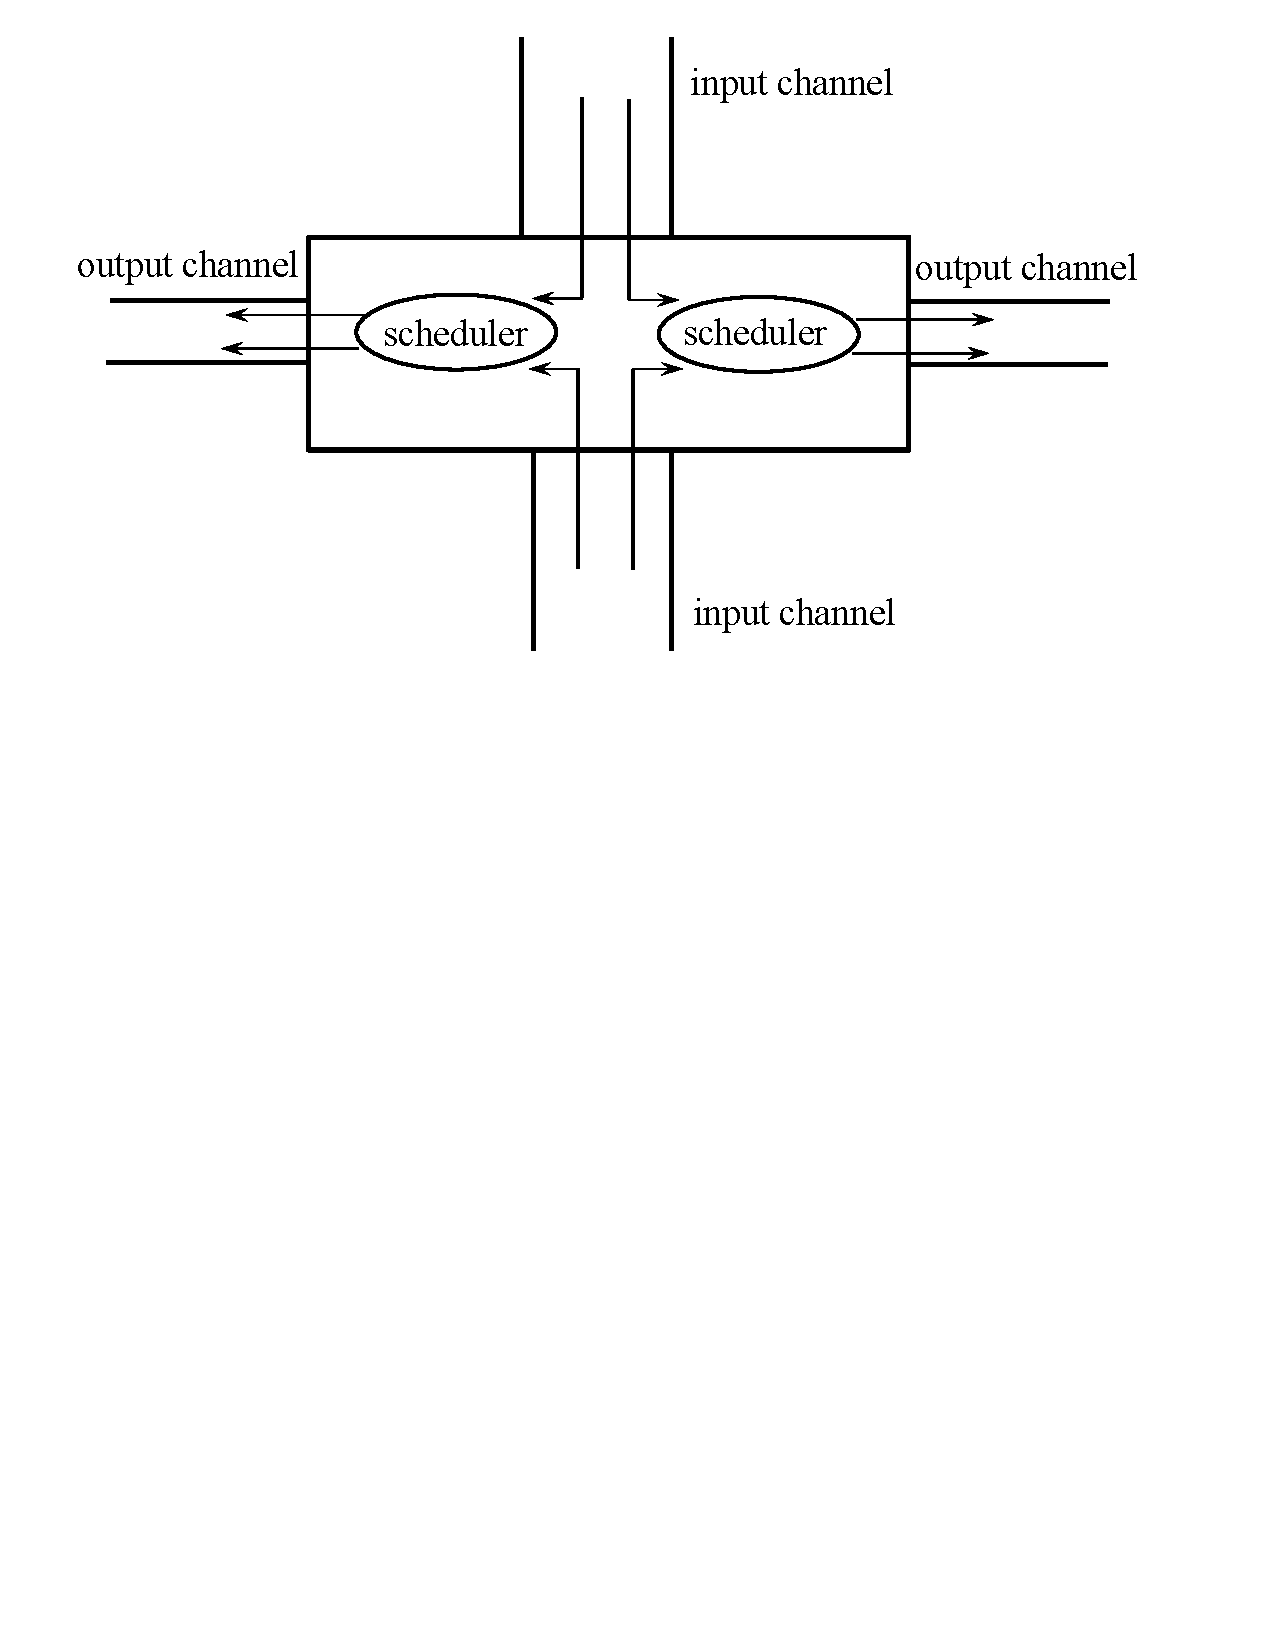
\includegraphics[scale=0.8]{paper/Fig1}

\caption{\textbf{Schedulers and Channels}}


\label{fig:fig1} 
\end{figure}


\noindent \rule{1\columnwidth}{0.5mm}

We adopt the following notation for each flow $f$.

\begin{center}
\begin{tabular}{rl}
$R_{f}$  & data rate reserved for flow $f$. \tabularnewline
$p_{f,i}$  & $i^{th}$ packet of $f$, $i\geq1$. \tabularnewline
$L_{f,i}$  & length of packet $p_{f,i}$. \tabularnewline
$L_{f}^{max}$  & maximum packet length of $f$. \tabularnewline
$L^{max}$  & maximum packet length of all flows. \tabularnewline
$A_{f,i}$  & arrival time of $p_{f,i}$. \tabularnewline
$E_{f,i}$  & exit time of $p_{f,i}$. \tabularnewline
$C$  & bandwidth of the output channel. \tabularnewline
\end{tabular}
\par\end{center}

Consider a constant-rate (CR) fluid server%
\footnote{Fluid servers can forward, during any time interval, an arbitray number
of bits from any subset of its input flows. They are for reference
only and cannot be implemented. This is in contrast to packet schedulers
which are used in practice and can only forward one packet at a time.%
} whose input is a set of flows, among them $f$. Let this server forward
the bits of each input flow $f$ at exactly its reserved rate $R_{f}$.
Such a fluid server is defined in Fig. \ref{fig:CR}, where $B(t)$
are the \emph{backlogged flows} at time $t$, i.e., flows with bits
remaining to be forwarded, and $\psi_{f,CR}(t)$ is the bit rate given
to flow $f$ at time $t$.

\begin{figure}[H]
\noindent \rule{1\columnwidth}{0.5mm}\textbf{\centerline{ CR Server}}

\begin{tabbing}

\noindent \textbf{let $B(t)$ be the set of backlogged flows at time
$t$;}\\
\textbf{for every flow $f$, }\\
\textbf{\taba if $f\in B(t)$, then}\\
\textbf{\tabb$\psi_{f,CR}(t)=R_{f}$}\\
\textbf{ \taba else}\\
\textbf{ \tabb$\psi_{f,CR}(t)=0$ }

\end{tabbing}

\textbf{\rule{1\columnwidth}{0.5mm}}

\noindent \textbf{\caption{\textbf{Constant-rate fluid server}}
}

\textbf{\label{fig:CR} }
\end{figure}


Let us define $S_{f,i,CR}$ as the \emph{start-time} of packet $p_{f,i}$
at the constant-rate server and $F_{f,i,CR}$ as the \emph{finishing
time}. They can be computed recursively as follows, where $S_{f,1,CR}=A_{f,1}$.
\begin{eqnarray}
S_{f,i,CR} & = & \mbox{max}(A_{f,i},\ F_{f,i-1,CR})\ \ \mbox{\ensuremath{i>1}}\nonumber \\
F_{f,i,CR} & = & S_{f,i,CR}+\frac{L_{f,i}}{R_{f}}\ \ \mbox{\ensuremath{i\geq1}}\label{eq:F-def}
\end{eqnarray}
Note that $F_{f,i,CR}$ is the value used by the Virtual Clock scheduling
protocol to assign priorities to its packets \citep{VC-Lam,VC-Lixia}.

Assume that a packet scheduler $s$ forwards the packets of an input
flow $f$ at a rate of at least $R_{f}$. Then, each packet $p_{f,i}$
exits scheduler $s$ not much later than its finishing time at $CR$,
i.e., $F_{f,i,CR}$. These packet schedulers are referred to as \emph{rate-guaranteed
schedulers} \citep{Cobb-Flow-Theory-ToN,leaveintime,NOSSDAV-95-Vin}.
More formally, a scheduler $s$ is a rate-guaranteed scheduler iff,
for every input flow $f$ of $s$ and every $i$, $i\geq1$, 
\begin{equation}
E_{f,i,s}\leq F_{f,i,CR}+\delta_{f,s}\label{eq:E-e2e}
\end{equation}
for some constant $\delta_{f,s}$. For many protocols, such as Virtual
Clock \citep{VC-Lam,VC-Lixia} and Weighted Fair Queuing \citep{GPS-Parekh}
(and their many variations), 

\begin{equation}
\delta_{f,s}=L_{s}^{max}/C_{s}
\end{equation}
i.e., packets exit by their finishing time in $CR$ plus at most the
time to transmit the largest packet size. In this case, admission
control is simple%
\footnote{Other protocols have a {\em rate-independent delay} \citep{leaveintime,KGShin94}:
where $\delta_{f,s}$ could be negative. This allows for a smaller
per-hop delay, but makes the admission control test quite complex.
Such protocols are outside the scope of this paper. %
}, the sum of the reserved rates of all the flows through $s$ must
be at most $C$.


\section{Rate Equalization}

In this section, the Rate-Equalization fairness which was presented
in \citep{Cobb-REQ} is discussed. On occasions, the bandwidth of
a channel is not fully utilized. This occurs either because existing
flows are transmitting at a rate that is below their reserved rate,
or because the sum of the reserved rates of the flows is less than
the output channel's bandwidth. Under these conditions, it is possible
for a flow to temporarily exceed its reserved rate, in an attempt
to take advantage of bandwidth that is not being used by other flows.
The source of the flow can determine if there is unused bandwidth
by receiving implicit feedback from the network, in particular, that
its packets are experiencing an end-to-end delay that is smaller than
expected.

The manner in which unallocated bandwidth is distributed among flows
varies from one scheduling protocol to another. We refer to this distribution
of unallocated bandwidth as the \emph{fairness} method of the protocol,
and it is the main focus of this paper.

Some protocols, like Virtual Clock (VC) \citep{VC-Lixia}\citep{VC-Lam},
do not address fairness. In VC, each packet $p_{f,i}$ is labeled
with its virtual finishing time, $F_{f,i,CR}$ (see (\ref{eq:F-def})),
and packets are forwarded by the scheduler in order of increasing
labels. A consequence of this is that, if a flow exceeds its reserved
rate, it may later be denied service by the scheduler, for a duration
proportional to the time the flow exceeded its rate \citep{Cobb-TS-Scheduling-ToN}.
This is potentially unbounded. The exit bound in Equation (\ref{eq:E-e2e})
still holds, however, because VC is a rate-guaranteed scheduler.

Other rate-guaranteed protocols, such as Weighted Fair Queuing (WFQ)
\citep{GPS-Parekh} and its variants \citep{Hui-Hierarchical-WFQ}
\citep{Cobb-TS-Scheduling-ToN} \citep{SCFQ-Golestani} \citep{Hui-WF2Q},
distribute the unallocated bandwidth among flows in proportion to
their reserved rate. Specifically, the effective rate $\psi_{f}$
that is given to flow $f$ (i.e., the rate at which the scheduler
actually forwards the packets of flow $f$) is 
\begin{equation}
\psi_{f}(t)=\frac{C}{\left(\sum_{g\in B(t)}R_{g}\right)}\cdot R_{f}\geq R_{f}\label{eq:WFQ-Share}
\end{equation}
where $B(t)$ are the backlogged flows at time $t$ (i.e., those flows
with a non-empty queue) and $C$ is the capacity of the output channel
of the scheduler.

Consider another flow $g$ with lesser reserved bandwidth, e.g., $R_{f}=2\cdot R_{g}$.
From (\ref{eq:WFQ-Share}), it can be easily shown that 
\[
(\psi_{f}-R_{f})=2\cdot(\psi_{g}-R_{g})
\]
That is, the manner in which unused bandwidth is allocated to backlogged
flows is proportional to the reserved rate of the flow. Hence, the
fairness method of WFQ favors flows with a higher reserved rate.

\noindent The intuition behind WFQ's fairness method is as follows.
If a flow has a reserved rate that is greater than that of other flows,
it implies that the user who generates the flow is paying a greater
price for the network service, and thus, should receive a greater
share of the unallocated bandwidth.

In \citep{Cobb-REQ}, we presented an alternative fairness method
in which the overall objective is to give every flow the same effective
rate, provided enough unallocated bandwidth is available. This will
result in a value for the effective rate $\psi_{f}$ that is different
from the one given in Equation (\ref{eq:WFQ-Share}). The intuition
behind it is the following. Every flow will be guaranteed its reserved
rate $R_{f}$. However, flows whose applications are rate-adaptive
could reserve the minimum rate possible to satisfy their QoS requirements,
and thus minimize expense. Any additional bandwidth is given to those
flows that need it the most, i.e., those with the least reserved rate.

A more detaied description is as follows. First, at all times, the
effective rate of any flow $f$, $\psi_{f}$, is at least its reserved
rate, $R_{f}$. I.e., $R_{f}\leq\psi_{f}$. Next, consider another
flow $g$, where $R_{f}<R_{g}$. By definition, $R_{g}\leq\psi_{g}$.
In our method, if enough unallocated bandwidth is available, $\psi_{f}$
will increase until it becomes equal to $R_{g}$, and thus, $\psi_{f}$
will become equal to $\psi_{g}$. Thus, flows with lower reserved
rates will ``catch up'' to flows with larger reserved rates.

Assume that more unallocated bandwidth remains. In this case, the
remaining unallocated bandwidth will be distributed equally between
$f$ and $g$, maintaining the relationship $\psi_{f}=\psi_{g}$.
If there exists another flow $h$, where $R_{h}>R_{g}$, then $\psi_{f}$
and $\psi_{g}$ increase equally until they reach $R_{h}$ (assuming
enough bandwidth remains), and hence, $\psi_{f}=\psi_{g}=\psi_{h}$.

To summarize, our fairness method attempts to give all flows the same
effective rate. However, in doing so, the requirement of $R_{f}\leq\psi_{f}$
for all $f$ must be preserved at all times.

We next describe our fairness method in a more formal way by introducing
a rate equalization fluid server, which will then be emulated as close
as possible by a packet scheduler.


\section{Rate-Equalization Server and Scheduler}

Packet scheduling algorithms that provide fairness, such as WFQ and
some of its variants, describe their fairness method via a virtual
fluid server. The packet scheduler then mimics the fluid server as
much as possible. The fluid server and the packet scheduler have the
same input flows. Both have an output channel, and both of these channels
have equal capacity.

What distinguishes the fluid server from the packet scheduler is the
manner in which it forwards bits. Once the packet scheduler begins
to transmit a packet, the transmission of the packet cannot be preempted.
The fluid server, on the other hand, can concurrently forward an arbitrary
number of bits from a group of flows. This, of course, is bounded
by the capacity (bits/sec.) of the output channel.


\subsection{Fluid Server}

In light of our earlier discussion on fairness, we define the rate-equalization
(EQ) fluid server as follows. Let $\psi_{f,EQ}(t)$ be the instantaneous
bit rate given to flow $f$ by the fluid server. This value is computed
as shown in Figure \ref{fig:EQ-server}. If $\psi_{f,EQ}(t)$ does
not change during an interval $[t_{1},t_{2}]$, then the total number
of bits of $f$ forwarded during this interval is $\psi_{f,EQ}(t_{1})\cdot(t_{2}-t_{1})$.

The steps shown in Figure \ref{fig:EQ-server} are as follows. First,
the set $B(t)$ of backlogged flows (i.e., with bits remaining to
be forwarded) is determined. Obviously, a non-backlogged flow receives
a rate of zero. All other flows are then arranged in increasing order
of their reserved rate. Then, the index $j$ is found such that 
\[
R_{b_{j}}\leq\frac{C-\sum_{k=j+1}^{m}R_{b_{k}}}{j}<R_{b_{j+1}}
\]
In this manner, if the higher rate flows $b_{j+1},\ldots,b_{m}$ receive
exactly their reserved rate, then there is enough remaining bandwidth
that can be equally shared among the lower rate flows 

\begin{figure}[H]
\rule{1\columnwidth}{0.5mm} \centerline{\textbf{EQ Server}}

\begin{tabbing}

\textbf{Let $B(t)$ be the set of backlogged flows at time $t$;}\\
\textbf{for every flow $f$, }\\
\textbf{\taba if $f\notin B(t)$, then}\\
\textbf{ \tabb $\psi_{f,EQ}(t)=0$}\\
\textbf{ \taba else}\\
\textbf{ \tabb let $b_{1},b_{2},\ldots,b_{m}$ be the flows of $B(t)$}\\
\textbf{ \tabb \ \ ordered by increasing $R$;}\\
\textbf{ \tabb let $j$, $1\leq j\leq m$, be the largest index such
that}\\
\textbf{ \tabc ${\displaystyle R_{b_{j}}\leq\frac{C-\sum_{k=j+1}^{m}R_{b_{k}}}{j}<R_{b_{j+1}}}$;}\\
\textbf{ \tabb let ${\displaystyle R_{EQ}=\frac{C-\sum_{k=j+1}^{m}R_{b_{k}}}{j}}$;}\\
\textbf{ \tabb for each $k$, $1\leq k\leq j$, }\\
\textbf{ \tabc $\psi_{f,EQ}(t)=R_{EQ}$;}\\
\textbf{ \tabb for each $k$, $j+1\leq k\leq m$,}\\
\textbf{ \tabc $\psi_{f,EQ}(t)=R_{b_{k}}$;}

\end{tabbing}

\noindent \rule{1\columnwidth}{0.5mm} 

\caption{Rate equalization fluid server\label{fig:EQ-server}}
\end{figure}
\begin{figure}[t]
\centerline{ \setlength{\unitlength}{0.75in} \begin{picture}(4,2.6)(-0.25,-0.25)
%(x,y)(x0,y0)  x,y size of box x0y0 coordinate of botton left corner
%axis
\linethickness{1pt} \put(0,0){\line(1,0){3.5}} \put(0,0){\line(0,1){2.4}}
\put(0,-0.25){0} \put(0.95,-0.25){1} \put(1.95,-0.25){2}
\put(2.95,-0.25){3} \put(-0.3,0.75){40} \put(-0.3,1.55){80}
\put(-0.35,2.35){120} %ticks horizontal
\put(1,0){\line(0,1){0.1}} \put(1,0){\line(0,-1){0.1}}
\put(2,0){\line(0,1){0.1}} \put(2,0){\line(0,-1){0.1}}
\put(3,0){\line(0,1){0.1}} \put(3,0){\line(0,-1){0.1}}
%ticks vertical
\multiput(-0.15,0.2)(0,0.2){12}{ \line(1,0){0.2} } %draw lines for the first two seconds
%only three flows
\put(0,0.8){\line(1,0){2}} \put(0.8,0.4){$\psi_{f_{1}}=40$}
\put(0,1.6){\line(1,0){2}} \put(0.8,1.2){$\psi_{f_{2}}=40$}
\put(0,2.4){\line(1,0){2}} \put(0.8,2){$\psi_{f_{3}}=40$}
%dotted line at 2
\linethickness{0.5pt} \multiput(2,0)(0,0.2){12}{\line(0,1){0.12}}
\linethickness{1pt} %draw lines after the first two seconds
\put(2,0.5){\line(1,0){0.8}} \put(2.05,0.2){$\psi_{f_{1}}=25$}
\put(2,1){\line(1,0){0.8}} \put(2.05,0.7){$\psi_{f_{2}}=25$}
\put(2,1.6){\line(1,0){0.8}} \put(2.05,1.25){$\psi_{f_{3}}=30$}
\put(2,2.4){\line(1,0){0.8}} \put(2.05,1.95){$\psi_{f_{4}}=40$}
%dotted line at 2.8
\linethickness{0.5pt} \multiput(2.8,0)(0,0.2){12}{\line(0,1){0.12}}
\linethickness{1pt} %after 2.8, only three flows
\put(2.8,0.8){\line(1,0){0.7}} \put(3,0.35){$\psi_{f_{2}}=40$}
\put(2.8,1.6){\line(1,0){0.7}} \put(3,1.15){$\psi_{f_{3}}=40$}
\put(2.8,2.4){\line(1,0){0.7}} \put(3,1.95){$\psi_{f_{4}}=40$}
\end{picture} } \caption{Fluid server example.}


\label{fig:Fluid-Example} 
\end{figure}


Consider the following example, which is illustrated in Fig. \ref{fig:Fluid-Example}.
Let $C=120$ bits/sec.. There are four flows, $f_{1}\ldots f_{4}$,
and all packets are 100 bits long. Let $R_{f_{1}}=10$ bits/sec.,
$R_{f_{2}}=20$ bits/sec., $R_{f_{3}}=30$ bits/sec., and $R_{f_{4}}=40$
bits/sec.. Note that $\sum_{i=1}^{4}R_{f_{i}}=100$ bits/sec., leaving
20 bits/sec. unallocated.

Assume that at time 0, one packet of $f_{1}$ arrives, two packets
of $f_{2}$ arrive, and two packets of $f_{3}$ arrive. At time 2
secs., one packet of $f_{4}$ arrives.

At time zero, flows $f_{1}$, $f_{2}$, and $f_{3}$ have bits in
their queues. Since $C=120$, there is enough capacity for all three
flows to receive the same effective bandwidth of $\psi=40$ bits/sec..
At time 2, a packet from $f_{4}$ arrives. The total reserved rates
of the flows is 100 bits/sec., leaving only 20 bits/sec. to equalize
the rates among the flows. Equalizing $f_{1}$ to $f_{2}$ requires
10 bits/sec.. The remaining 10 bits/sec. are distributed equally between
$f_{1}$ and $f_{2}$, but are not enough to increase their effective
rates up $R_{f_{3}}$. We thus end with $\psi_{f_{1}}=\psi_{f_{2}}=25$
bits/sec. This leaves $\psi_{f_{3}}=R_{f_{3}}=30$ bits/sec., and
$\psi_{f_{4}}=R_{f_{4}}=40$ bits sec.

At time $2\frac{4}{5}$, the last bit of the packet of $f_{1}$ exits,
so only three flows have a non-empty queue. Again, all remaining flows
are given an effective bandwidth of 40 bits/sec. In the similar fashion
one can compute the remainder of the example.


\chapter{Logarithmic Rate Equalization Scheduler}

We next overview the packet scheduler for rate-equalization which
we presented in \citep{Cobb-REQ}, where more details can be found.

In general, the purpose of a fluid server is to guide the packet scheduler
in the order it chooses to forward packets. Typically, \citep{Cobb-Universal-Timestamp-CN}\citep{GPS-Parekh}\citep{RP-Fair-Servers-ToN},
for every pair of packets, $p_{1}$ and $p_{2}$, if $p_{1}$ finishes
service in the fluid server before $p_{2}$ finishes service, then
the packet scheduler will forward $p_{1}$ before $p_{2}$. I.e.,
the packet scheduler tries to emulate the behavior of the fluid server
as much as possible. This emulation, of course, is not perfect, because
the packet scheduler can only forward one packet at a time, while
the fluid server can forward bits of multiple flows (and hence multiple
packets) at once.


\section{Packet Scheduler}

For most fluid servers \citep{Cobb-Universal-Timestamp-CN}\citep{GPS-Parekh}\citep{RP-Fair-Servers-ToN},
at the moment a packet arrives, the exit time that this packet will
have from the fluid server is unknown. This is because the bit rate
at which the packet will be served depends not only on the packets
currently in the system, but also on packets that are yet to arrive.

In consequence, when a packet $p_{f,i}$ arrives into a packet scheduler,
the scheduler assigns to the packet a {\em virtual exit time} $T_{f,i}$
(see \citep{GPS-Parekh} for details on computing this value), such
that, for any other packet $p_{g,j}$, $T_{f,i}\leq T_{g,j}$ iff
the exit time of $p_{f,i}$ from the fluid server is at most the exit
time of $p_{g,j}$. Packets are then forwarded in order of their virtual
exit times. Thus, the packet scheduler forwards packets in the same
order in which they are forwarded by the fluid server.

A rate-equalizing fluid server, however, does not have this order-preserving
property. That is, if two packets $p_{f,i}$ and $p_{g,j}$ are received,
not only can't their exit time from the fluid server be determined,
but also their relative exit times cannot be determined. I.e., which
of $p_{f,i}$ or $p_{g,j}$ exits first depends on the future arrival
of packets.

The reason for not having this property is that the relative effective
bandwidth, $\psi_{g}/\psi_{f}$, does not remain constant in rate-equalization.
Actually, {\em not} preserving this ratio is one of the objectives
of rate-equalization. Hence, when packets $p_{g,j}$ and $p_{f,i}$
arrive, the scheduler is unable to determine which one will exit the
fluid server first.

From the above, the rate equalization packet scheduler (PEQ) cannot
assign a virtual exit time $T$ to each packet. Instead, we opted
in \citep{Cobb-REQ} to assign a real-time deadline, $D_{f,i,PEQ}$,
to each packet $p_{f,i}$. The deadline is an {\em upper bound}
on the exit time of $p_{f,i}$ from the fluid server. To obtain this
upper bound, we take advantage of the fact that both the fluid server
and the packet scheduler have the same input flows and the same output
channel capacity. This allows the packet scheduler to keep track of
the behavior of the fluid server. The upper bound is as follows.

Let $S_{f,i,EQ}$ be the starting time of $p_{f,i}$ in the fluid
server, i.e., when its first bit begins service. Note that scheduler
PEQ cannot compute this value when $p_{f,i}$ arrives. However, at
time $t$, where $t\geq S_{f,i,EQ}$, PEQ is aware of this value,
because it can keep track of the behavior of the server. Thus, the
deadline of $p_{f,i}$ is set to 
\begin{equation}
D_{f,i,PEQ}=S_{f,i,EQ}+\frac{L_{f,i}}{R_{f}}.
\end{equation}
Then, packets are forwarded in order of this deadline.

Note that since $\psi_{f}\geq R_{f}$, the above is a true upper bound
on the exit time from the fluid server. Furthermore, since scheduler
$PEQ$ cannot compute this value until time $S_{f,i,EQ}$, $p_{f,i}$
is not added to the queue of schedulable packets until this time.

The detailed behavior of the scheduler is shown in Figure \ref{fig:PEQ-scheduler}.
More detais can be found in \citep{Cobb-REQ}, including bounds on
the difference between a packet's exit time from the scheduler and
from the fluid server.

\textbf{}
\begin{figure}[H]
\noindent \rule{1\columnwidth}{0.5mm} \centerline{\textbf{PEQ Scheduler} }

\noindent \begin{tabbing}

\noindent \textbf{upon receiving a packet $p_{f,i}$,}\\
\textbf{ \taba $D_{f,i,PEQ}=\infty$;}\\
\textbf{  if output channel is idle at time $t$,}\\
\textbf{ \taba model the behavior of $EQ$ up to time $t$;}\\
\textbf{ \taba let $p_{f,i}\in\mbox{Active}(t)$ iff $t\geq S_{f,i,EQ}$;}\\
\textbf{ \taba for each $p_{f,i}\in\mbox{Active}(t)$,}\\
\textbf{ \taba $D_{f,i,PEQ}=S_{f,i,EQ}+L_{f,i}/R_{f}$;}\\
\textbf{ \taba let $D_{g,j,PEQ}=\mbox{min}\{D_{f,i,PEQ}\,\,|\,\, p_{f,i}\in\mbox{Active}(t)\}$;}\\
\textbf{ \taba forward $p_{g,j}$ to the output channel. }\end{tabbing} 

\textbf{\label{fig:PEQ-scheduler} \rule{1\columnwidth}{0.5mm} }

\textbf{\caption{\textbf{Packetized rate equalization scheduler}}
}

\end{figure}



\section{Roadblocks to Efficient Implementation}

Recall that our objective is to find an approximation algorithm that
will require $O(\log(n))$ processing for receiving and transmitting
a packet, where $n$ is the number of flows in the system. Our scheduling
protocol resembles WFQ in the sense that we also have a fluid server,
and the packet scheduler attempts to emulate it as close as possible.

For many years, the best implementation of WFQ had $O(n)$ complexity.
This was due to the overhead of computing the virtual time associated
with the arrival time of a packet. The virtual time grows inversely
proportional to the number of flows backlogged in the fluid server.
The $O(n)$ complexity arises because many flows could become not
backlogged in a very short period of time.

Several approximations with $O(\log(n))$ complexity, such as Leap-Forward-VC
\citep{leapforward}, Time-Shift Scheduling \citep{Cobb-TS-Scheduling-ToN},
and WFQ+ \citep{Hui-WF2Q}, provided a rough approximation of the
virtual time. Other approaches reduced the complexity even further
to $O(1)$ by sophisticated variations on the classical round-robin
algorithm \citep{SRR}\citep{G-3}\citep{Stratified}\citep{FRR}\citep{GRR}\citep{VWQGRR}.
All of these provided the same type of fairness as WFQ, i.e., extra
bandwidth is allocated in proportional to the reserved rate.

After many years of only having an $O(n)$ implementation, an $O(\log(n))$
implementation of WFQ was presented in \citep{WFQlogN}. This required
the introduction of a complex search structure that organized the
``breaking points'' in the virtual time into a search tree. Crucial
to making this implementation possible is that the ratio of the effective
rates, $\psi_{g}/\psi_{f}$ for any pair of backlogged flows, remained
the same regardless of the arrival or departure of packets from other
flows.

However, the ratio mentioned above is not constant in rate-equalization
scheduling. In fact, it can vary significantly. To see this, consider
again Figure \ref{fig:EQ-server}. You can consider the set of backlogged
flows to always be divided into two subsets: those flows whose effective
rate is their reserved rate, and those flows whose effective rates
are all the same due to unused bandwidth. The amount of unused bandwidth
in turn depends on how many flows are backlogged, which, like in WFQ,
can vary signnificantly in a very short period of time. This causes
many flows to change from one of these two subsets to another, which
in turn drastically changes the ration of effective rates.

For these reasons, a technique similar to the one in \citep{WFQlogN}
is not directly applicable. Although we have not proven a lower bound,
we speculate that a precise implementation cannot be done in $O(\log(n))$
time. We thus search for an approximation to the fluid server of rate-equalization
that runs in $O(\log(n))$ time. Our approximation, presented below,
is quite different from that of earlier works mentioned above due
to our significantly different method of defining fairness.


\section{Dual-Mode Scheduling}

From the above discussion, backlogged flows in the fluid server can
be cosidered to be in one of two disjoint subsets: {\em enhanced
flows}, whose effective rate is greater than their reserved rate
and all members have the same effective rate, and {\em unenhanced
flows}, whose effective rate is simply their reserved rate. This
motivates our first packet scheduler design, presented in Section
\ref{subsec:Flow-Migration-Scheduler}. Although intuitive, this first
attempt is not efficient. We then present our final scheduler design
in Section \ref{subsec:Static-Flow-Scheduler}


\subsection{Flow-Migration Scheduler}

\label{subsec:Flow-Migration-Scheduler}

\begin{figure}[H]
\begin{centering}
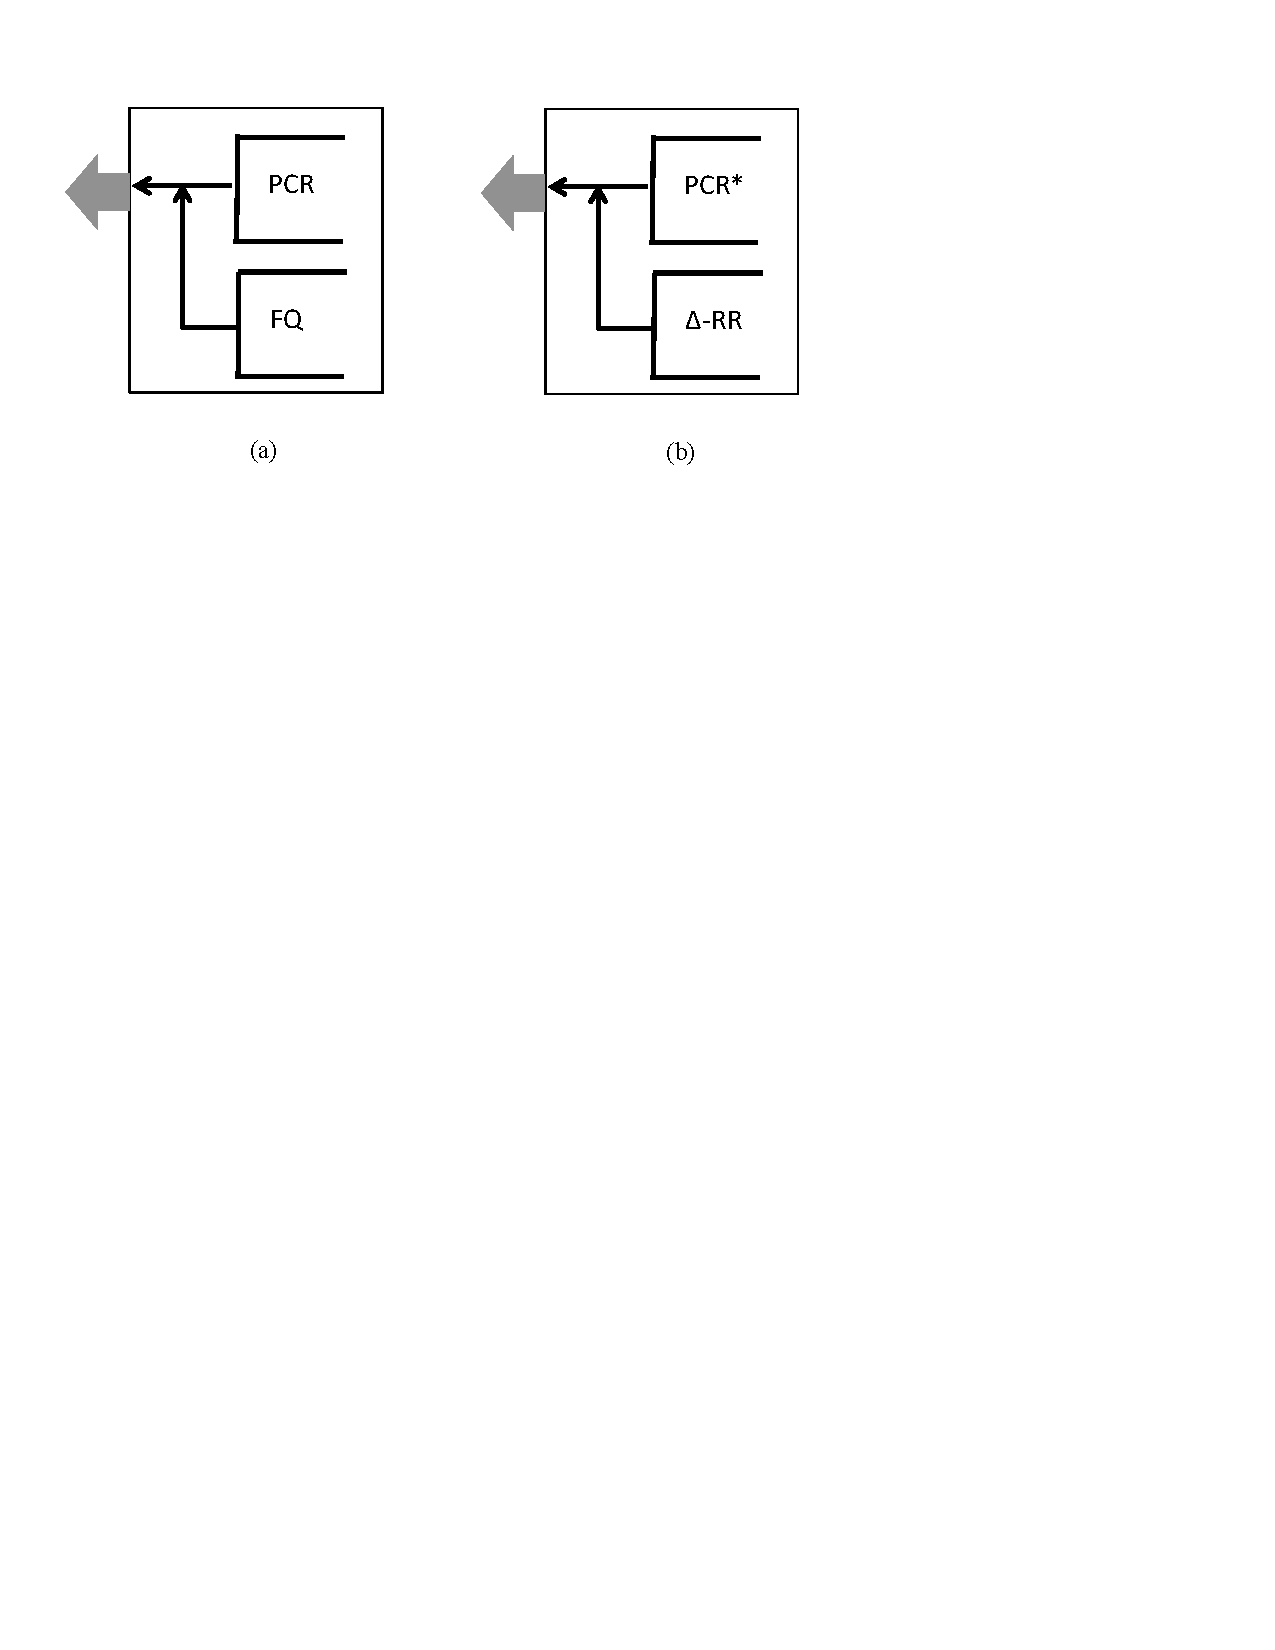
\includegraphics{paper/FigDual}
\par\end{centering}



\caption{Dual-Mode Scheduling}


\label{fig:Dual-Mode} 
\end{figure}


\textbf{}
\begin{figure}[H]
\noindent \textbf{\rule{1\columnwidth}{0.5mm} \centerline{} PCR
Scheduler} \begin{tabbing} 

\noindent \textbf{Let $B(t)$ be the set of backlogged flows at time
}$t$ 

\noindent upon receiving a packet $p_{f,i}$,\\
 %\tea $S_{f,i,CR} = \mbox{max}(A_{f,i},F_{f,i,CR})$;\\
\taba $D_{f,i,PCR}=F_{f,i,CR}$;\\
 \\
 if output channel is idle at time $t$,\\
 \taba let $p_{f,i}\in\mbox{Active}(t)$ iff $t\geq S_{f,i,CR}$;\\
 \taba if $\mbox{Active}(t)\neq\emptyset$ then\\
 \tabb let $D_{g,j,PCR}=\mbox{min}\{D_{f,i,PCR}\,\,|\,\, p_{f,i}\in\mbox{Active}(t)\}$;\\
 \tabb forward $p_{g,j}$ to the output channel. \end{tabbing} 

\label{fig:PCR} \rule{1\columnwidth}{0.5mm} \caption{\textbf{Packetized constant-rate scheduler}}
\end{figure}


Consider Figure \ref{fig:Dual-Mode}(a). The service required for
an unenhanced flow $f$ is simply a constant rate $R_{f}$. This is
provided by a packetized constant rate scheduler (PCR), which is described
in more detail in Figure \ref{fig:PCR}. It is similat to the Virtual
Clock protocol \citep{VC-Lam}, except that it does not allow flows
to exceed their reserved rate. Note that this scheduler is non-work-conserving,
i.e., there are times when its queues are non-empty yet it does not
have any packets considered 'active', so it remains idle. Enhanced
flows, on the other hand, have to be served in an equal manner. This
is best accomplished by a fair-queuing (FQ) scheduler, also shown
in Figure \ref{fig:Dual-Mode}(a).

We thus have two schedulers, one for each type of flow. Priority is
given to the PCR scheduler. I.e., when the output channel becomes
idle, the PCR scheduler is queried for the next packet to be transmitted.
Only if the PCR scheduler is unable to provide a packet (due to its
queues being empty or all packets being 'inactive'), then the packet
transmitted is chosen from the FQ scheduler. Both of these schedulers
can be implemented in $O(\log(n))$ time per packet arrival/departure
(FQ using the method of \citep{WFQlogN}).

The above method should work, provided the membership in the enhanced
and unenhanced flow sets remains constant. However, their membership
depends on unallocated bandwidth. An increase in unallocated bandwidth
enhances more flows, and a decrease unenhances some flows.

Unallocated bandwidth comes from two sources: from bandwidth that
is not reserved by any flow, and from flows that have temporarilly
stopped creating packets (empty queues). The former is relatively
stable, and changes are predictable (when flows are added or removed).
In this case, the appropriate movement of flows between the schedulers
can be done before a new flow is accepted or removed from the system.
The latter, i.e., queues becoming empty, cannot be predicted, and
may cause large changes in flow assignments to the two schedulers.
This is particularly true if the flows whose queue becomes empty have
a large reserved bandwidth. Thus, moving flows from one scheduler
to the other is not efficient, which prompts us to present below our
final version of the scheduler.


\subsection{Static-Flow-Assignment Scheduler}

%%%%%%%%%%%%%%%%%%%%%%%%%%%%%%%%%
\label{subsec:Static-Flow-Scheduler}

\begin{figure}[H]
\noindent \rule{1\columnwidth}{0.5mm} \centerline{\textbf{A-PEQ
Scheduler}} \begin{tabbing} 

\noindent \textbf{upon receiving a packet $p_{f,i}$,}\\
\textbf{ \taba add $p_{f,i}$ to the queue of $f$, $Q_{f}$;}\\
\textbf{ if output channel is idle at time $t$,}\\
\textbf{ }\taba \textbf{model the behavior of $PCR^{*}$ to dequeue
a packet; }\\
\taba\textbf{ let $p_{f,i}$ be the packet chosen by $PCR^{*}$ ;}\\
\taba\textbf{ let $\rho_{min}=\mbox{min}\{\rho_{g}\,\,|\,\, Q_{g}\neq\emptyset\}$;}\\
\taba\textbf{ if $Q_{f}\neq\emptyset$ then}\\
\tabb\textbf{ dequeue and forward a packet from flow $f$;}\\
\tabb\textbf{ $\rho_{f}=\mbox{min}(\rho_{f}+1,\rho_{min}+\Delta)$;}\\
\taba\textbf{ else}\\
\tabb \textbf{let $g$ satisfy $\rho_{g}=\rho_{min}$;}\\
\textbf{\tabb forward the next packet of flow $g$;}\\
\textbf{\tabb $\rho_{g}=\rho_{g}+1$;}\end{tabbing}\textbf{ }

\textbf{\rule{1\columnwidth}{0.5mm} \label{fig:A-PEQ-Scheduler}\caption{\textbf{Approximate packetized rate equalization scheduler}}
}
\end{figure}


Our final protocol, {\em Approximate Packetized rate Equalization}
(A-PEQ), is shown in detail in Figure \ref{fig:A-PEQ-Scheduler},
with an abstract view in Figure \ref{fig:Dual-Mode}(b). For this
implementation, we make the simplifying assumption that all packets
of all flows have an equal size, L.%
\footnote{We will investigate eliminating this restriction in future work.%
} There are three major differences from the previous scheduler.

First, {\em all flows take part in both schedulers}. This solves
the problem of having to move a large number of flows between the
schedulers in a short period of time.

Second, the scheduler PCR{*} differs from PCR as follows. PCR{*} assumes
that every flow always has packets available (even if its queue is
empty). When it chooses a packet from flow $f$ for transmission,
it checks the queue of $f$. If it is empty, then the packet transmitted
is instead a packet chosen by $\Delta$-RR. Eventhough $f$ did not
transmit a packet, PCR{*} updates its state about $f$ as if indeed
it had transmitted a packet from $f$.

Third, instead of FQ, we have a modified round-robin scheduling, which
we denote $\Delta$-RR. Each flow $f$ has a round number $\rho_{f}$
in $\Delta$-RR. When $\Delta$-RR is asked to forward a packet, it
chooses it as follows.
\begin{itemize}
\item If $\Delta$-RR is called because PCR{*} is unable to transmit a packet,
then $\Delta$-RR chooses a packet from the backlogged flow {\em
with the least round-number}, and increases the flow's round number
by one. 
\item If PCR{*} is able to transmit a packet from a flow $f$, then the
round-number of $f$ is increased by one, {\em even though} $\Delta$-RR
{\em did not output a packet}. 
\end{itemize}
The motivation for the above choices is as follows. Consider two flows
$f$ and $g$, where $f$ has a large reserved rate (always unenhanced
in the fluid server) and $g$ a small reserved rate (always enhanced
in the fluid server). All unenhanced flows, such as $f$, transmit
packets from PCR{*} at a high rate, so their round numbers in $\Delta$-RR
are higher than those of other flows. The slower flows, such as $g$,
are served in round-robin order, and thus receive the same bandwidth.

Consider now two slow flows $g$ and $h$, with $g$ having a greater
reserved rate than $h$. Note that through their respective packet
transmissions at PCR{*}, the round number of $g$ grows faster than
$h$'s. Nonetheless, both flows receive about the same behavior from
$\Delta$-RR. This is because the unused bandwidth at PCR{*} causes
$\Delta$-RR to serve the slowest flows, such as $h$, first, which
allows these flows to reach the same round numbers as other flows,
such as $g$.

One final detail remains. Assume the round number of flow $f$, due
to its large reserved rate, grows much larger than that of other flows.
Then, assume enough bandwidth becomes available to make $f$ an enhanced
flow in the fluid server. However, due its large round number, $f$
will not receive service in $\Delta$-RR for a long time. To avoid
this, we place a bound, $\Delta$, on the difference between the round
number of any flow and the minimum round number of any backlogged
flow, as indicated in Figure \ref{fig:A-PEQ-Scheduler}.

The bound $\Delta$ is a tunable parameter of the system. If it is
too large, enhanced flows may not receive their due bandwith, and
if it is too small, bandwidth may be wasted on unenhanced flows.


\section{Performance Bounds}

In this section, we outline some of the upper bounds on the performance
of the A-PEQ scheduler. We first note that A-PEQ is a rate-guaranteed
scheduler. However it’s upper bound on the exit time is slightly greater
than that of Relation \ref{eq:exit-bound-wfq}, as follows. 
\begin{thm}
For every packet $p_{f,i}$ in the A-PEQ scheduler, 

\begin{equation}
E_{f,i,A-PEQ}\le F_{f,i,CR}+\frac{L}{R_{f}}
\end{equation}


The reason for the term $\frac{L}{R_{f}}$ , as opposed to the smaller
term $\frac{L}{C}$ comes from the $PCR*$ scheduler, due to the following.
$PCR*$ chooses f, and if it finds f’s queue, then control is passed
to ∆-RR, but at this very moment a packet from f arrives. Thus, the
packet has missed its scheduling opportunity in PCR{*}. 
\end{thm}
Next, the complexity of A-PEQ is as desired. 
\begin{thm}
Let n be the number of input flows to an A- PEQ scheduler. Then, the
time complexity of processing a received packet and the time complexity
of selecting a packet for transmission is packet O(log(n)). 

For PCR{*}, an O(log(n)) time implementation is possible using well-known
techniques, such as maintaining only one finishing time, $F_{f}$
, for each flow f , as opposed to maintaining one value per packet.
Also, maintaining a queue of flows that will become active at some
time t can be done using the methods discussed in \citep{Hui-WF2Q}.
Implementing ∆-RR is obviously $O(log(n))$, since it only needs to
maintain the smallest round number among the backlogged flows.
\end{thm}
Finally, note that, contrary to schedulers like WFQ and PEQ, A-PEQ
does not simulate the behavior of the virtual fluid server. Thus,
it is difficult, if not impossible, to provide an upper bound on the
difference in the exit time of a packet from the EQ fluid server and
the A-PEQ packet scheduler. This is why we provide simulations in
Chapter \ref{chap:Simulations-and-Results}, which evaluate how closely
A-PEQ approximates our initial $O(n)$ packet scheduler, PEQ. Nonetheless,
to argue that A-PEQ does provide the desired fairness, we have the
following.
\begin{thm}
Assume that starting from a time $t$, for each flow in an $A-PEQ$
scheduler, either its queue is always empty or always non-empty. Let
$b_{1},b_{2},...,b_{m}$ be the set of backlogged flows. Let $j$
be as defined in \ref{fig:A-PEQ-Scheduler}. Hence, flows $b_{1},\; b_{2},\;.....b_{j}$
are permanently enhanced in the fluid server, while flows $b_{j+1},...,b_{m}$
are permanently un-enhanced. Let $P(t_{1},t_{2},b_{k})$ be the number
of bits from flow $b_{k}$ transmitted by the $A-PEQ$ scheduler during
time interval $[t_{1},\; t_{2}]$. Finally, let

\begin{equation}
\Delta\;>\;\frac{R_{max}}{R_{min}}
\end{equation}


where $R_{max}$ and $R_{min}$ are the maximum and minimum reserved
rates among the backlogged flows. Then, \end{thm}
\begin{itemize}
\item For every $k$, $1\le k\le j$, as $t\lyxmathsym{′}$ increases,
$P(t,t\lyxmathsym{′},b_{k})$ converges to $REQ$, where $REQ$
is as defined in \ref{fig:EQ-server}. 
\item For every $k,\; j+1\;\le\; k\;\le\; m$, as $t\lyxmathsym{′}$ increases,
$P(t,t\lyxmathsym{′},b_{k})$ converges to $R_{b_{k}}$ .
\end{itemize}

\chapter{Simulations and Results}

\label{chap:Simulations-and-Results}

Our goal is to design a scheduler which provides fairness of EQ scheduler
in logarithmic time. In the previous chapter, we looked at the details
of A-PEQ scheduler. We proved that A-PEQ scheduler is a rate-guaranteed
which assures ateast the reserved amount of bandwidth to each flow
with a slightly higher value of upper bound. We claimed that it can
be implemented in logarithmic time, since both $PCR^{*}$ and $\Delta-RR$
can itself be implemented with logarithmic complexity using exiting
techniques. We also gave a formal proof that A-PEQ scheduler provides
the identical or similar fairness as EQ scheduler provided the state
of flows doesn't change in the system.

In case of schedulers like WFQ, there exists a corresponding fluid
server. If such cases, it is possible to compare the fairness of approximation
algorithms with the fairness providedd by the ideal server. However,
$A-PEQ$ doesn't emulate any such fluid server. To prove that despite
of lack of a fluid server, $A-PEQ$ does offer fairness which is similar
to $EQ$ scheduler, we run simulations to compare the behavior of
different schedulers. Fairness is contingent upon various factors
like:
\begin{itemize}
\item Traffic patterns
\item Number of flows in the system
\item Reservations by each flow
\end{itemize}
There are other factors as well which might affect the behavior of
the scheduling policy like packet drop probabilities, queue lengths
etc. However, for the sake of simplicity we didn't consider them during
simulations. To see the performance in possible practical scenarios,
we run a number of simulations in which same traffic patterns were
pushed through $WFQ$, $EQ$, $PEQ$ and finally through $A-PEQ$.
In the following section, we describe the simulation environment,
traffic patterns and assumptions used in the simulator. 


\section{Simulation Environment}

We simulate the behavior of a single scheduling node, with 30 input
flows. The total output channel capacity of the node is $165\; Mbytes/sec.$.
Each flow falls into exactly one of the following groups:

\begin{table}[H]
\begin{tabular}{|c|c|}
\hline 
Group Name & Description\tabularnewline
\hline 
\hline 
A & Generate packets at an average rate equal to their reserved rates\tabularnewline
\hline 
B & Generate packets at an average rate which is equal to half of their
reserved rates\tabularnewline
\hline 
C & Generate packets at a very high rate such that their queues are always
non-empty\tabularnewline
\hline 
\end{tabular}

\caption{Flow categories in simulation}
\end{table}


In all the simulation scenarios, each of the above mentioned groups
is:
\begin{itemize}
\item either empty
\item or non empty with exactly 10 flows
\end{itemize}
All the flow have their reserved rates in the scheduling node, which
are described below:
\begin{itemize}
\item Flows $A_{1}$ through $A_{10}$ correspond to group $A$ and have
a reserved rate of $1,\;2,\;.....,\;10\; Mbytes/sec.$ respectively.
E.g., flow $A_{1}$ generates packets at $1\; Mbyte/sec.$, flow $A_{2}$
gererates packets at rate of $2\; Mbytes/sec.$, and flow $A_{10}$
generates packets at a rate of $10\; Mbytes/sec.$.
\item Flows $B_{1}$ through $B_{10}$ correspond to group $B$ and have
a reserved rate of $1,\;2,\;.....,\;10\; Mbytes/sec.$ respectively.
E.g., flow $B_{1}$ generates packets at $0.5\; Mbyte/sec.$, flow
$B_{2}$ gererates packets at rate of $1\; Mbytes/sec.$, and flow
$B_{10}$ generates packets at a rate of $5\; Mbytes/sec.$.
\item Flows $C_{1}$ through $C_{10}$ correspond to group $C$ and have
a reserved rate of $1,\;2,\;.....,\;10\; Mbytes/sec.$ respectively.
Note that only flows in C can take advantage of unused bandwidth,
since flows in A and B create packets at the same rate (or lower)
than their reserved rate.
\end{itemize}
Other assumptions made are follows:
\begin{itemize}
\item All the queue lengths are considered to be of infinite size.
\item Drop probability of every packet is considered to be $0$.
\end{itemize}

\subsection{Overview of scenarios}

In the scheduling node, unused bandwidth may exist because of two
possible reasons described below


\subsubsection*{Unallocated (UA) bandwidth:}

Consider a system with only group $C$ flows. Then the total reserved
bandwith will be $55\; Mbytes/sec.$ which will result is $110\; Mbytes/sec.$
of unallocated bandwidth. We refer to this scenario as \textbf{UA}.


\subsubsection*{Allocated but unused (UU) bandwidth:}

Consider a system with all the three groups of flows. Then the total
reserved bandwith will be $165\; Mbytes/sec.$ which will result is
$0\; Mbytes/sec.$ of unallocated bandwidth. However, since flows
in group\textbf{ $B$ }generate packets at a rate half of their reserved
rates, it gives nearly $27.5\; Mbytes/sec.$ of unused bandwidth on
average which can be used by other flows. We refer to this scenario
as \textbf{U}U.

Thus, we simulate three general cases:
\begin{enumerate}
\item \textbf{UA}, which is achieved by including only flows in groups A
and C and thus leaves 1/3 of the channel bandwidth unallocated, 
\item \textbf{UU}, which is achieved by including all three flow groups
and leaves 1/6 of the bandwidth unused (B only uses half of its reserved
bandwith), and 
\item \textbf{UU + UA}, which is achieved by including only flows B and
C and leaves 1/3 + 1/6 of the channel bandwidth unallocated or unused. 
\end{enumerate}
Since we assume that flows in group $C$ always have non-empty queues,
their packet arrival distribution doesn't affect the behavior of the
system. However, for groups A and B, we simulate two kinds of arrival
distributions:
\begin{itemize}
\item constant packet arrival rate 
\item poisson arrival rate. 
\end{itemize}
We thus have a total of six different scenarios each for four different
scheduling algorithms. In the next sections, we present the results
of simulations.


\section{Simulation Results}


\subsection{UA, Poisson}

In this scenario, two groups $A$ and $C$ are considered and flows
in group $A$ have a poisson arrival process. In the plots, flows
with id $1,\;2,\;....,\;10$ correspond to flows $A_{1}$ through
$A_{10}$ and flows with id $11,\;12,\;....,\;20$ correspond to flows
$C_{1}$ through $C_{10}$.

\vspace{40pt}

\begin{figure}[H]
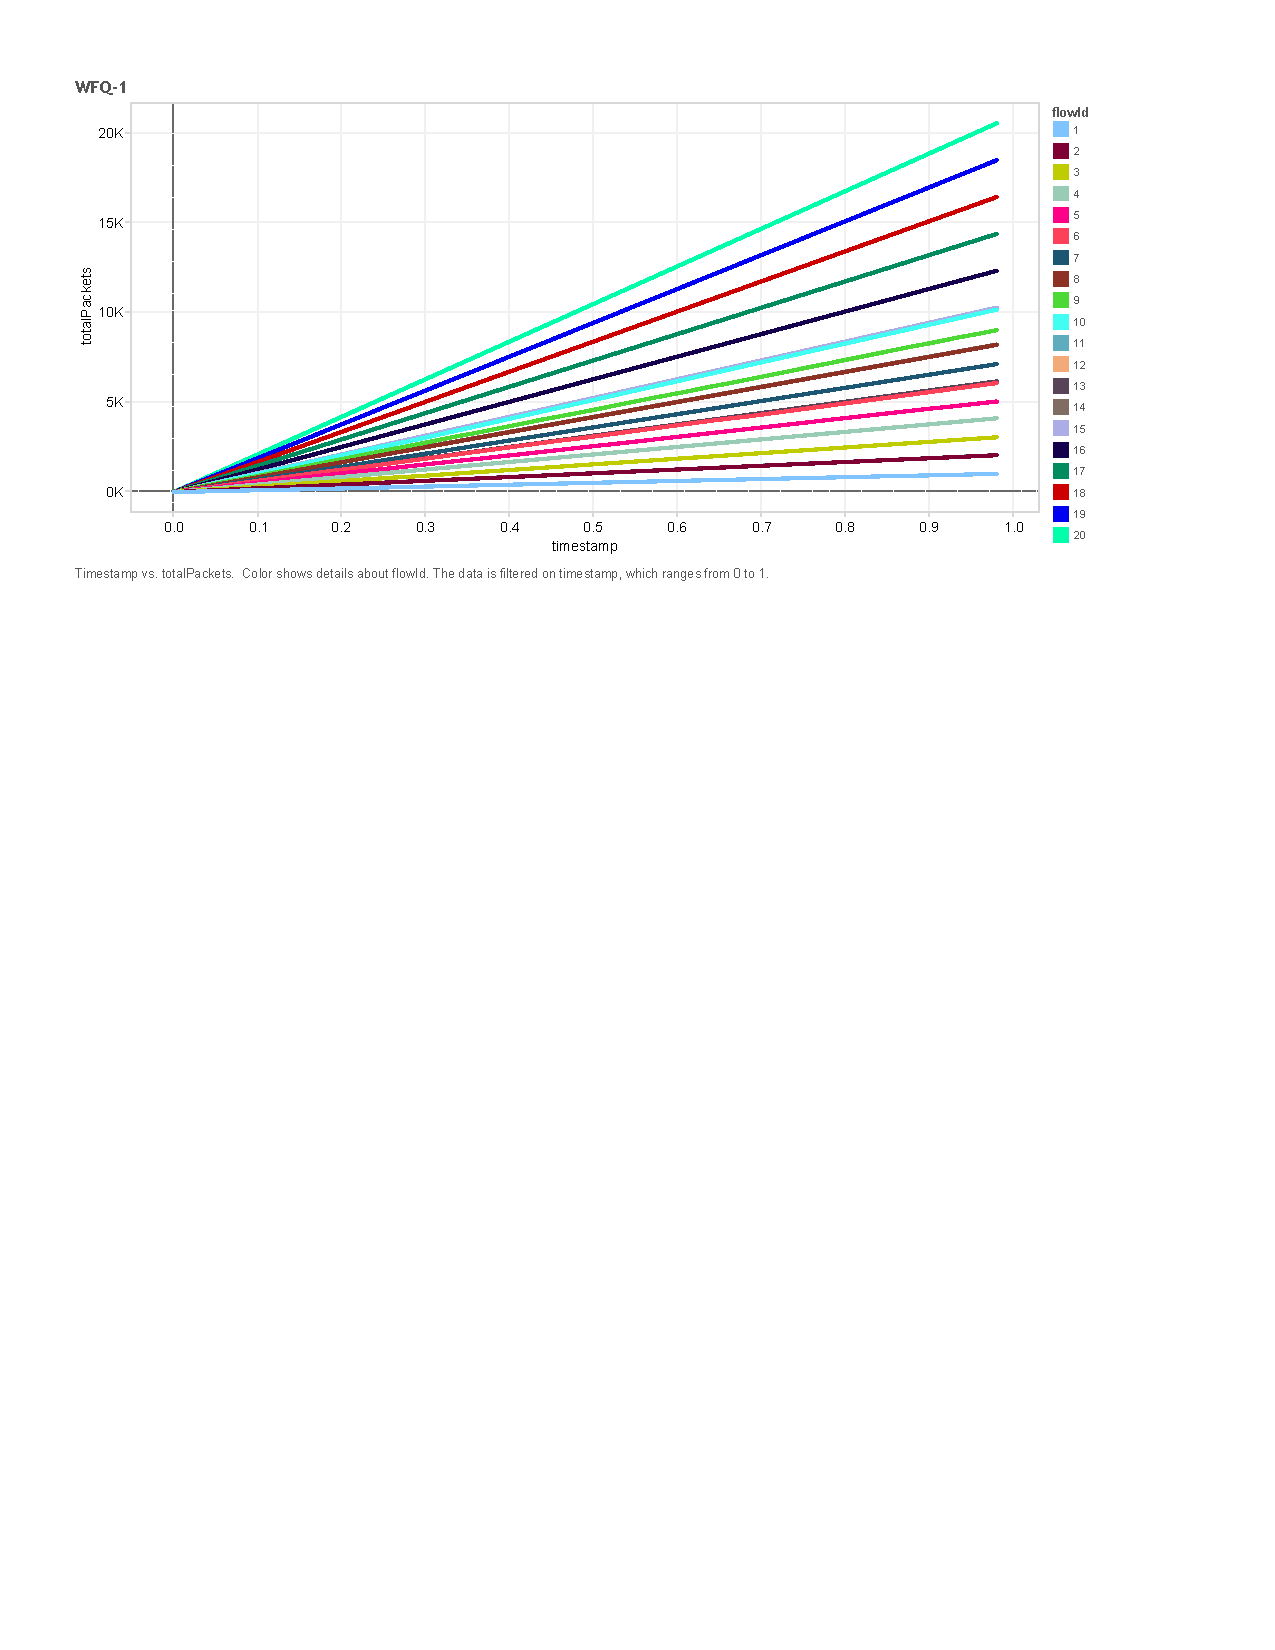
\includegraphics{plots/WFQ/WFQ-1}

\caption{UA, Poisson, WFQ\label{fig:UA,-Poisson,-WFQ}}
\end{figure}


Figure \ref{fig:UA,-Poisson,-WFQ} shows the behavior of $WFQ$. Since
flows $A_{1}$ through $A_{10}$ produce the packets at an average
rate equal to their reserved rates, they are not able to utilize the
extra bandwidth. However, since $C_{1}$ through $C_{10}$ are greedy
and always have non-empty queues, all of them get nearly twice the
bandwidth of the corresponding flows in group $A$, e.g. $C_{20}$
is able to transmit twice the number of packets than $A_{10}$ even
though both of them have a reserved rate of $10\; Mbytes/sec.$.

\pagebreak{}

Figure \ref{fig:UA,-Poisson,-EQ} shows the behavior of pure EQ scheduler.
Since flows $A_{1}$ through $A_{10}$ produce the packets at an average
rate equal to their reserved rates, they are not able to utilize the
extra bandwidth. However, since $C_{1}$ through $C_{10}$ are greedy
and always have non-empty queues, each of the group $C$ flows get
a bandwidth of nearly $11\; Mbytes/sec.$ and thus converge together
at a point above the plot of flow $A_{10}$.

\vspace{60pt}

\begin{figure}[H]
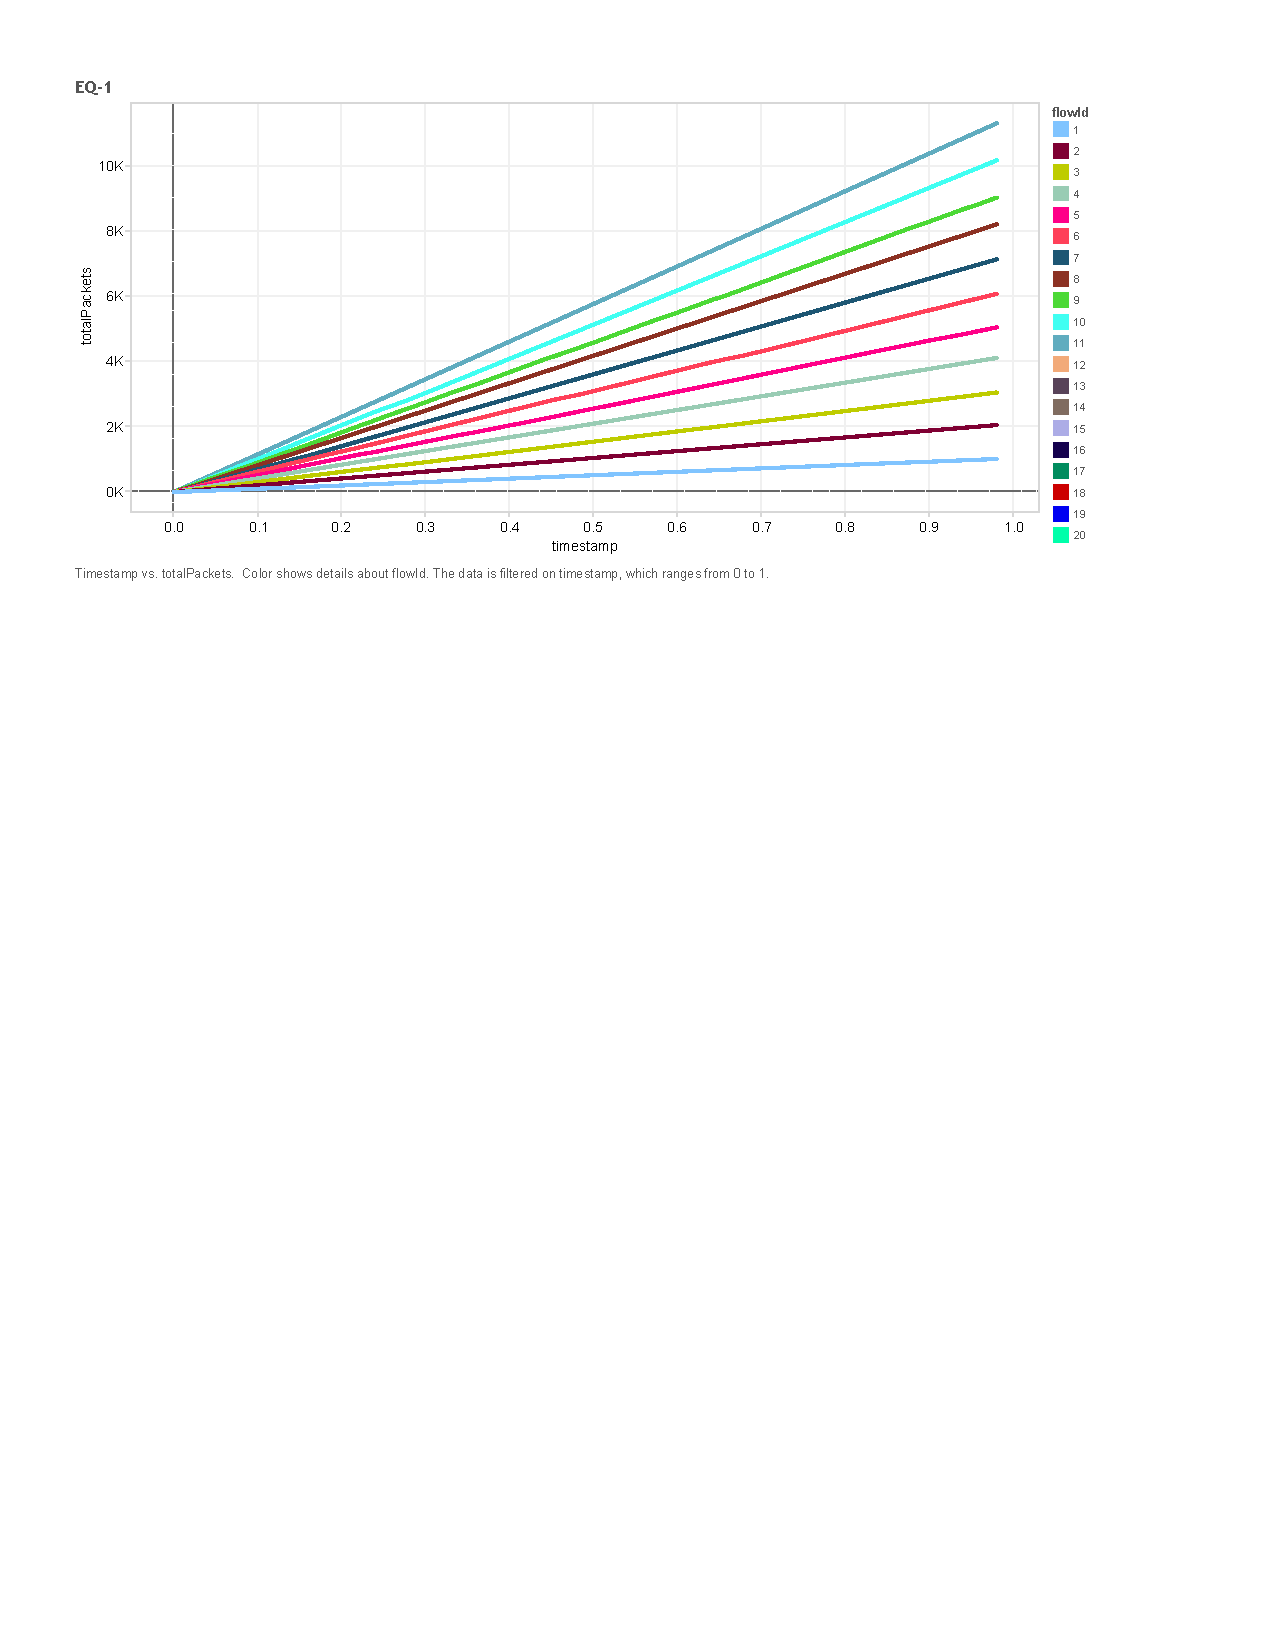
\includegraphics{plots/PEQ-EQ/EQ-1}

\caption{UA, Poisson, EQ \label{fig:UA,-Poisson,-EQ}}
\end{figure}


\pagebreak{}

Figure \ref{fig:UA,-Poisson,-PEQ} shows the behavior of PEQ scheduler.
As in the case of $EQ$, $C_{1}$ through $C_{10}$ are greedy and
always have non-empty queues, each of the group $C$ flows get a bandwidth
of nearly $11\; Mbytes/sec.$ on average and thus converge together
at a point above the plot of flow $A_{10}$. The plot is nearly identical
to that of $EQ$ scheduler.

\vspace{60pt}
\begin{figure}[H]
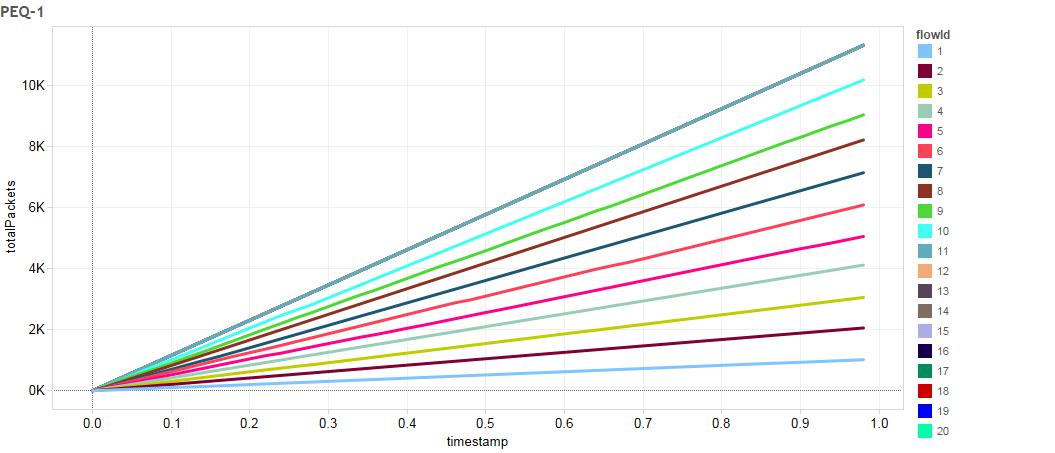
\includegraphics{plots/PEQ-EQ/PEQ-1}

\caption{UA, Poisson, PEQ \label{fig:UA,-Poisson,-PEQ} }
\end{figure}


\pagebreak{}

Figure \ref{fig:UA,-Poisson,-A-PEQ} shows the behavior of PEQ scheduler.
As in the case of $EQ$, $C_{1}$ through $C_{10}$ are greedy and
always have non-empty queues, each of the group $C$ flows get a bandwidth
of nearly $11\; Mbytes/sec.$ on average and thus converge together
at a point above the plot of flow $A_{10}$. The plot is nearly identical
to that of $EQ$ scheduler.

\vspace{60pt}
\begin{figure}[H]
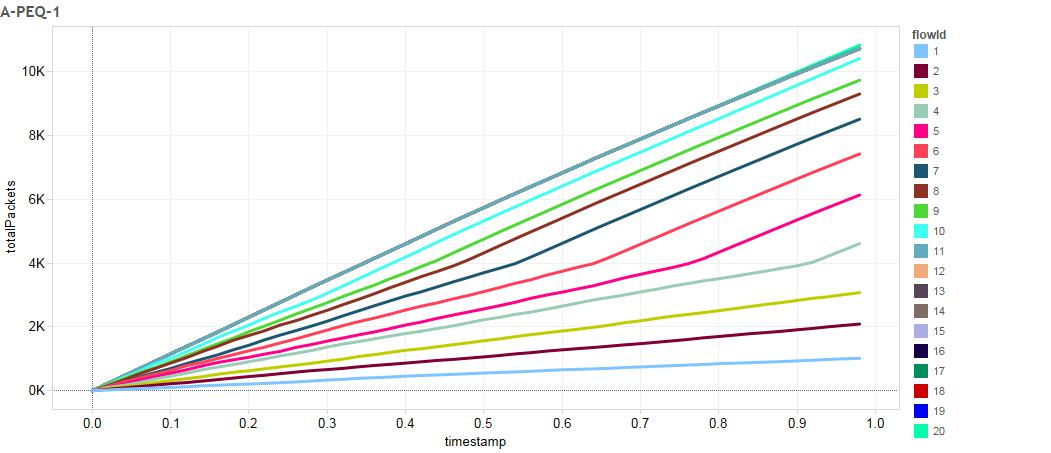
\includegraphics{plots/A-PEQ/A-PEQ-1}

\caption{UA, Poisson, A-PEQ \label{fig:UA,-Poisson,-A-PEQ} }
\end{figure}


\pagebreak{}


\subsection{UA, Constant Rate}

In this scenario, two groups $A$ and $C$ are considered and flows
in group $A$ have a poisson arrival process. In the plots, flows
with id $1,\;2,\;....,\;10$ correspond to flows $A_{1}$ through
$A_{10}$ and flows with id $11,\;12,\;....,\;20$ correspond to flows
$C_{1}$ through $C_{10}$.

\vspace{40pt}

\begin{figure}[H]
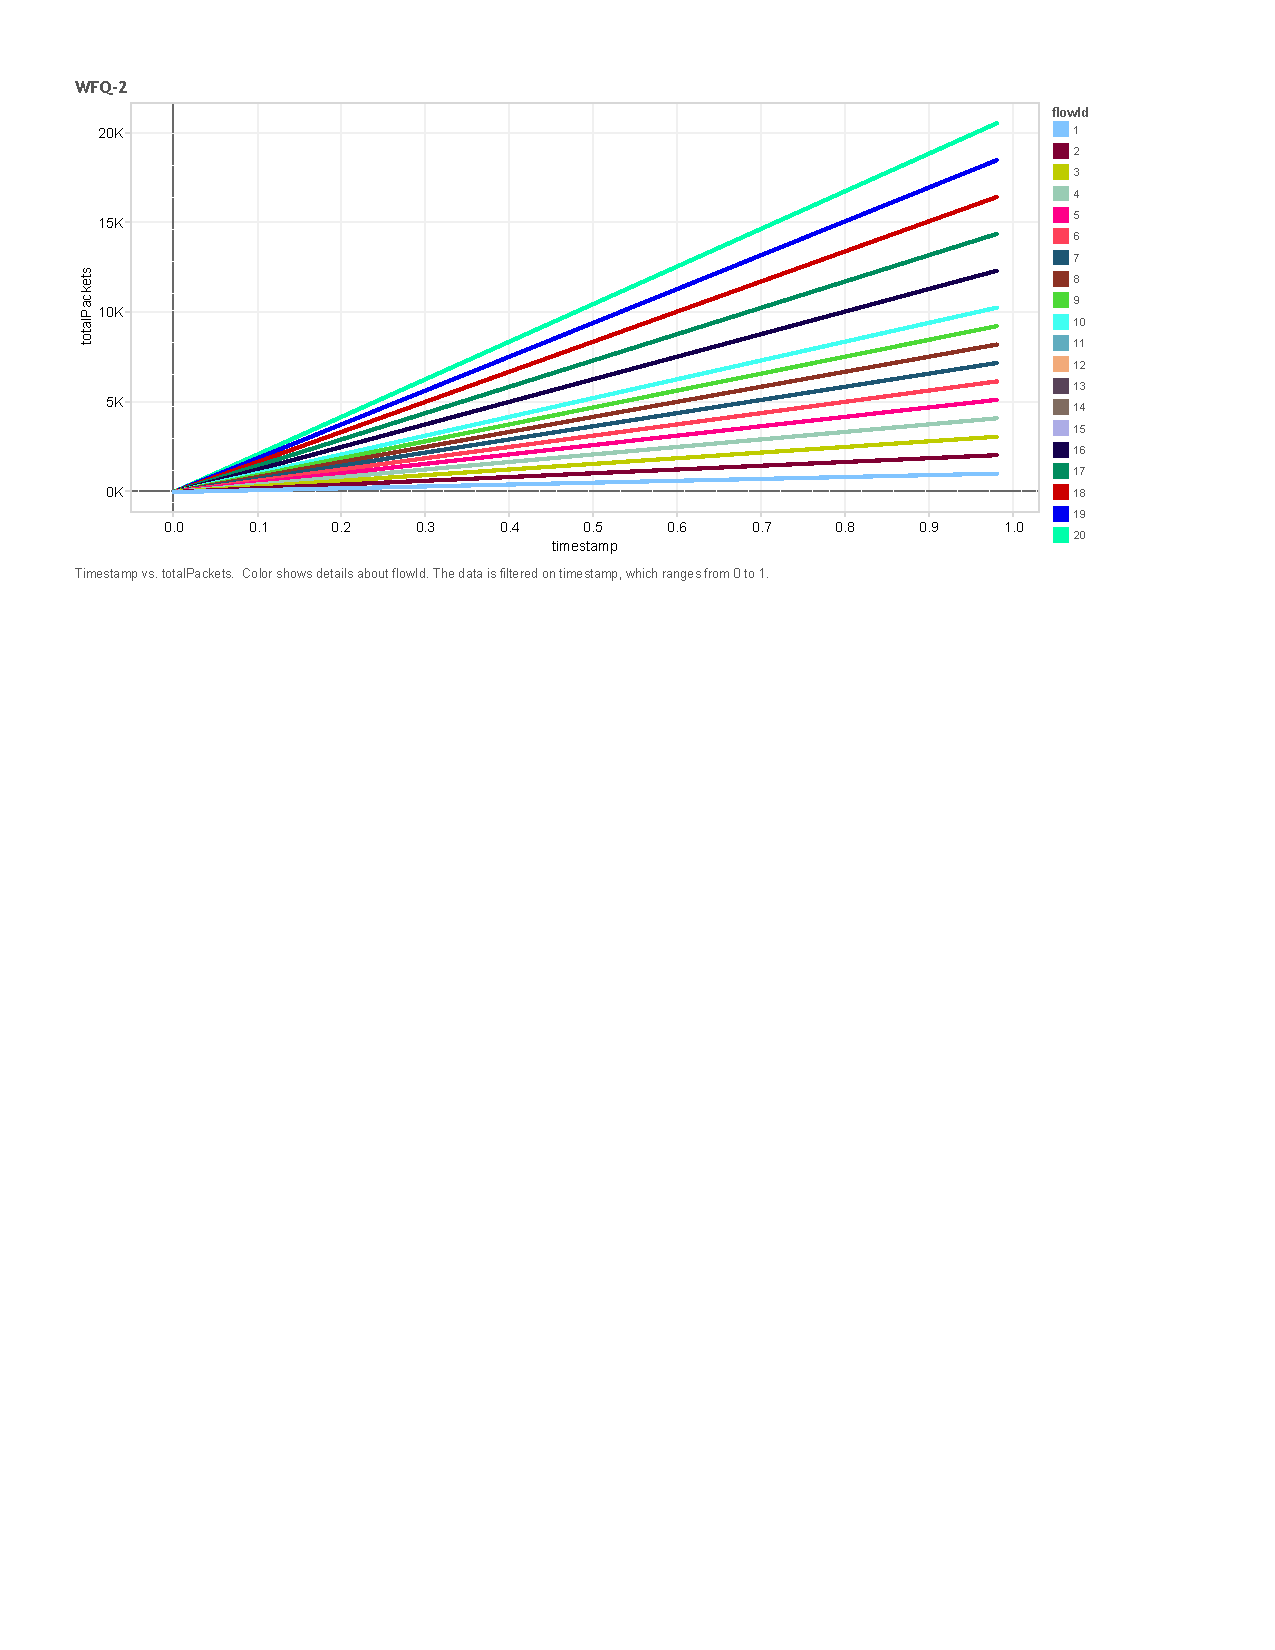
\includegraphics{plots/WFQ/WFQ-2}

\caption{UA, CR, WFQ\label{fig:UA,-CR,-WFQ}}
\end{figure}


Figure \ref{fig:UA,-CR,-WFQ} shows the behavior of $WFQ$. Since
flows $A_{1}$ through $A_{10}$ produce the packets at an average
rate equal to their reserved rates, they are not able to utilize the
extra bandwidth. However, since $C_{1}$ through $C_{10}$ are greedy
and always have non-empty queues, all of them get nearly twice the
bandwidth of the corresponding flows in group $A$, e.g. $C_{20}$
is able to transmit twice the number of packets than $A_{10}$ even
though both of them have a reserved rate of $10\; Mbytes/sec.$.

\pagebreak{}

Figure \ref{fig:UA,-CR,-EQ} shows the behavior of pure EQ scheduler.
Since flows $A_{1}$ through $A_{10}$ produce the packets at an average
rate equal to their reserved rates, they are not able to utilize the
extra bandwidth. However, since $C_{1}$ through $C_{10}$ are greedy
and always have non-empty queues, each of the group $C$ flows get
a bandwidth of nearly $11\; Mbytes/sec.$ and thus converge together
at a point above the plot of flow $A_{10}$.

\vspace{60pt}

\begin{figure}[H]
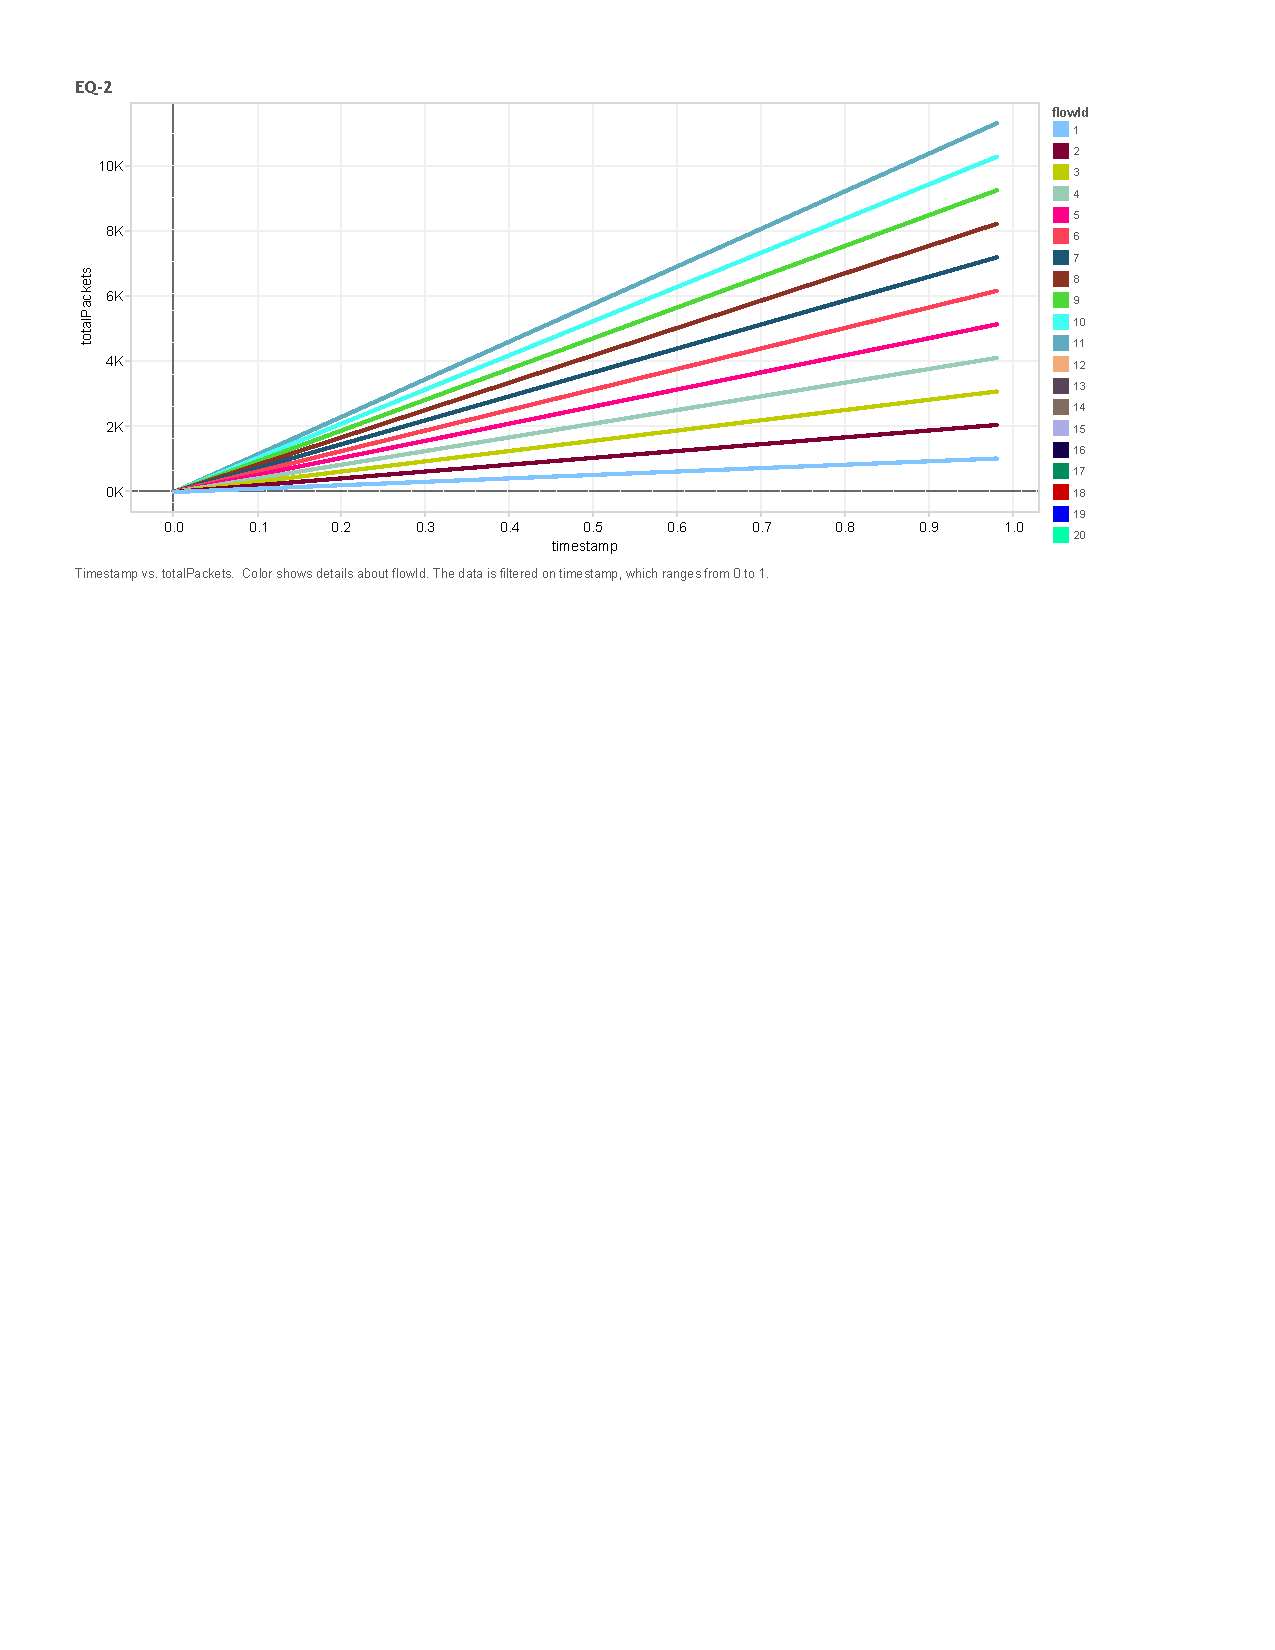
\includegraphics{plots/PEQ-EQ/EQ-2}

\caption{UA, CR, EQ \label{fig:UA,-CR,-EQ}}
\end{figure}


\pagebreak{}

Figure \ref{fig:UA,-CR,-PEQ} shows the behavior of PEQ scheduler.
As in the case of $EQ$, $C_{1}$ through $C_{10}$ are greedy and
always have non-empty queues, each of the group $C$ flows get a bandwidth
of nearly $11\; Mbytes/sec.$ on average and thus converge together
at a point above the plot of flow $A_{10}$. The plot is nearly identical
to that of $EQ$ scheduler.

\vspace{60pt}
\begin{figure}[H]
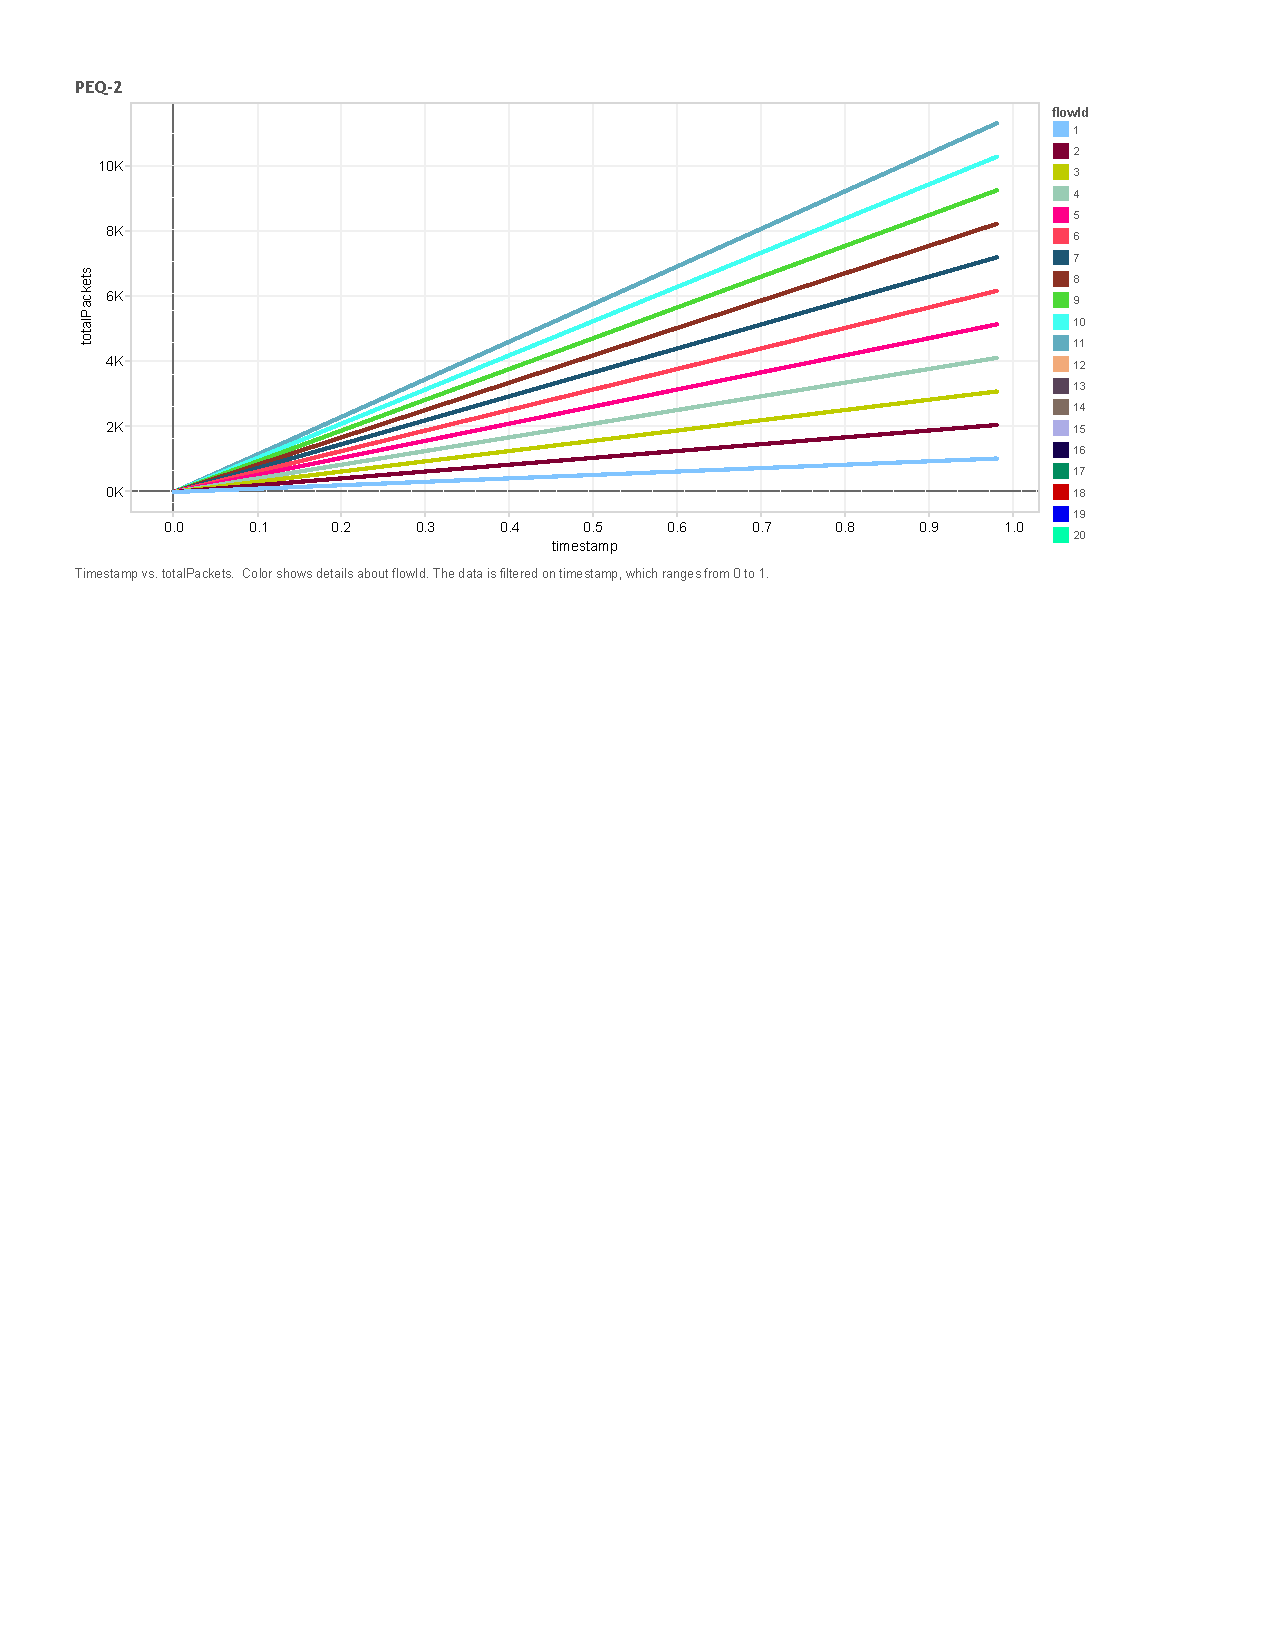
\includegraphics{plots/PEQ-EQ/PEQ-2}

\caption{UA, CR, PEQ \label{fig:UA,-CR,-PEQ} }
\end{figure}


\pagebreak{}

Figure \ref{fig:UA,-CR,-A-PEQ} shows the behavior of PEQ scheduler.
As in the case of $EQ$, $C_{1}$ through $C_{10}$ are greedy and
always have non-empty queues, each of the group $C$ flows get a bandwidth
of nearly $11\; Mbytes/sec.$ on average and thus converge together
at a point above the plot of flow $A_{10}$. The plot is nearly identical
to that of $EQ$ scheduler.

\vspace{60pt}
\begin{figure}[H]
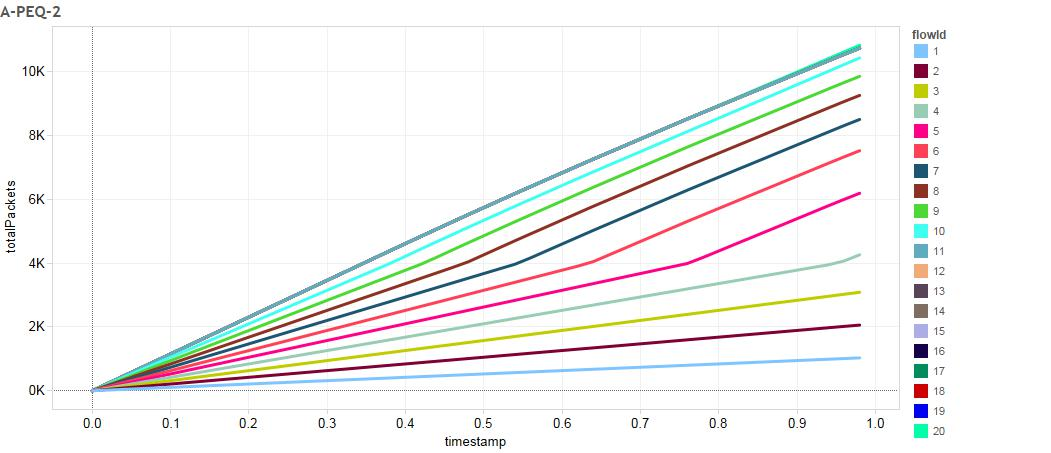
\includegraphics{plots/A-PEQ/A-PEQ-2}

\caption{UA, CR, A-PEQ \label{fig:UA,-CR,-A-PEQ} }
\end{figure}


\pagebreak{}


\subsection{UU, Poisson}

In this scenario, two groups $A$ and $C$ are considered and flows
in group $A$ have a poisson arrival process. In the plots, flows
with id $1,\;2,\;....,\;10$ correspond to flows $A_{1}$ through
$A_{10}$ and flows with id $11,\;12,\;....,\;20$ correspond to flows
$C_{1}$ through $C_{10}$.

\vspace{40pt}

\begin{figure}[H]
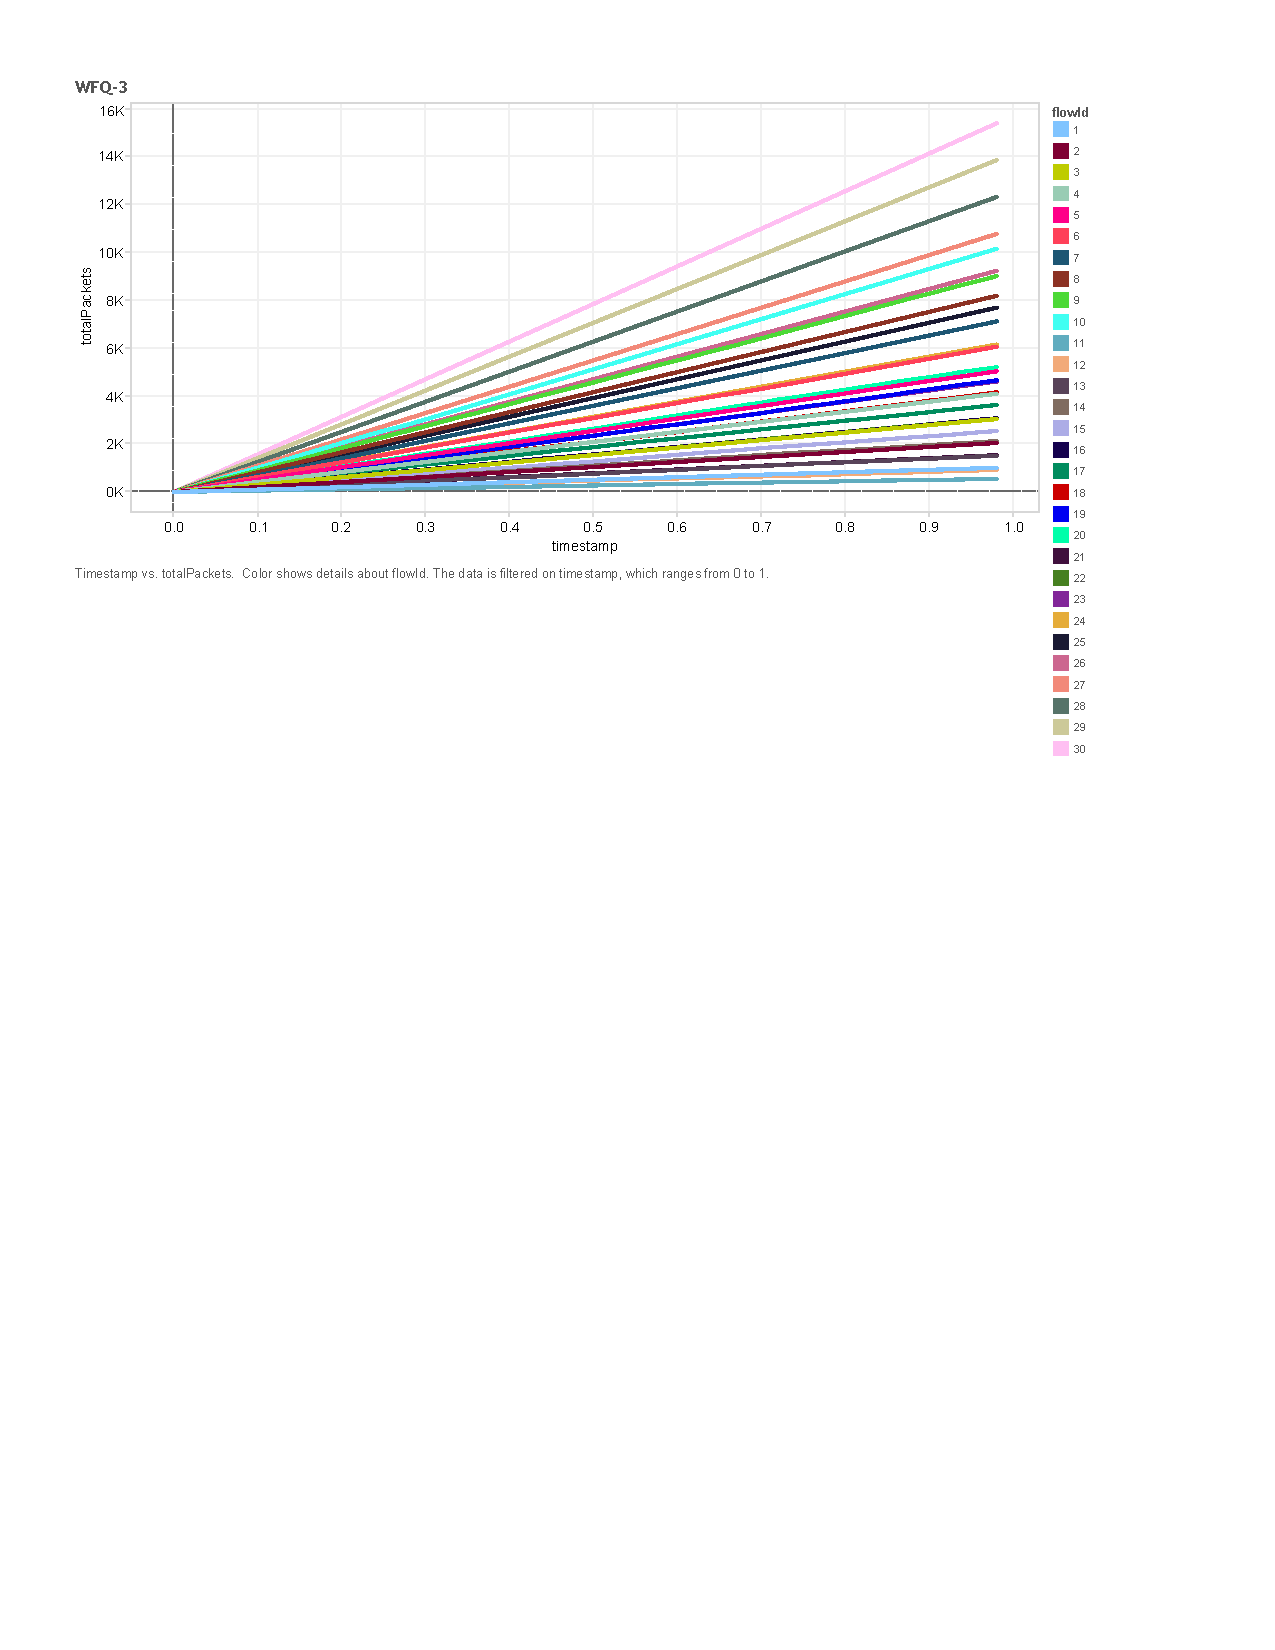
\includegraphics{plots/WFQ/WFQ-3}

\caption{UU, Poisson, WFQ\label{fig:UU,-Poisson,-WFQ}}
\end{figure}


Figure \ref{fig:UU,-Poisson,-WFQ} shows the behavior of $WFQ$. Since
flows $A_{1}$ through $A_{10}$ produce the packets at an average
rate equal to their reserved rates, they are not able to utilize the
extra bandwidth. However, since $C_{1}$ through $C_{10}$ are greedy
and always have non-empty queues, all of them get nearly twice the
bandwidth of the corresponding flows in group $A$, e.g. $C_{20}$
is able to transmit twice the number of packets than $A_{10}$ even
though both of them have a reserved rate of $10\; Mbytes/sec.$.

\pagebreak{}

Figure \ref{fig:UU,-Poisson,-EQ} shows the behavior of pure EQ scheduler.
Since flows $A_{1}$ through $A_{10}$ produce the packets at an average
rate equal to their reserved rates, they are not able to utilize the
extra bandwidth. However, since $C_{1}$ through $C_{10}$ are greedy
and always have non-empty queues, each of the group $C$ flows get
a bandwidth of nearly $11\; Mbytes/sec.$ and thus converge together
at a point above the plot of flow $A_{10}$.

\begin{figure}[H]
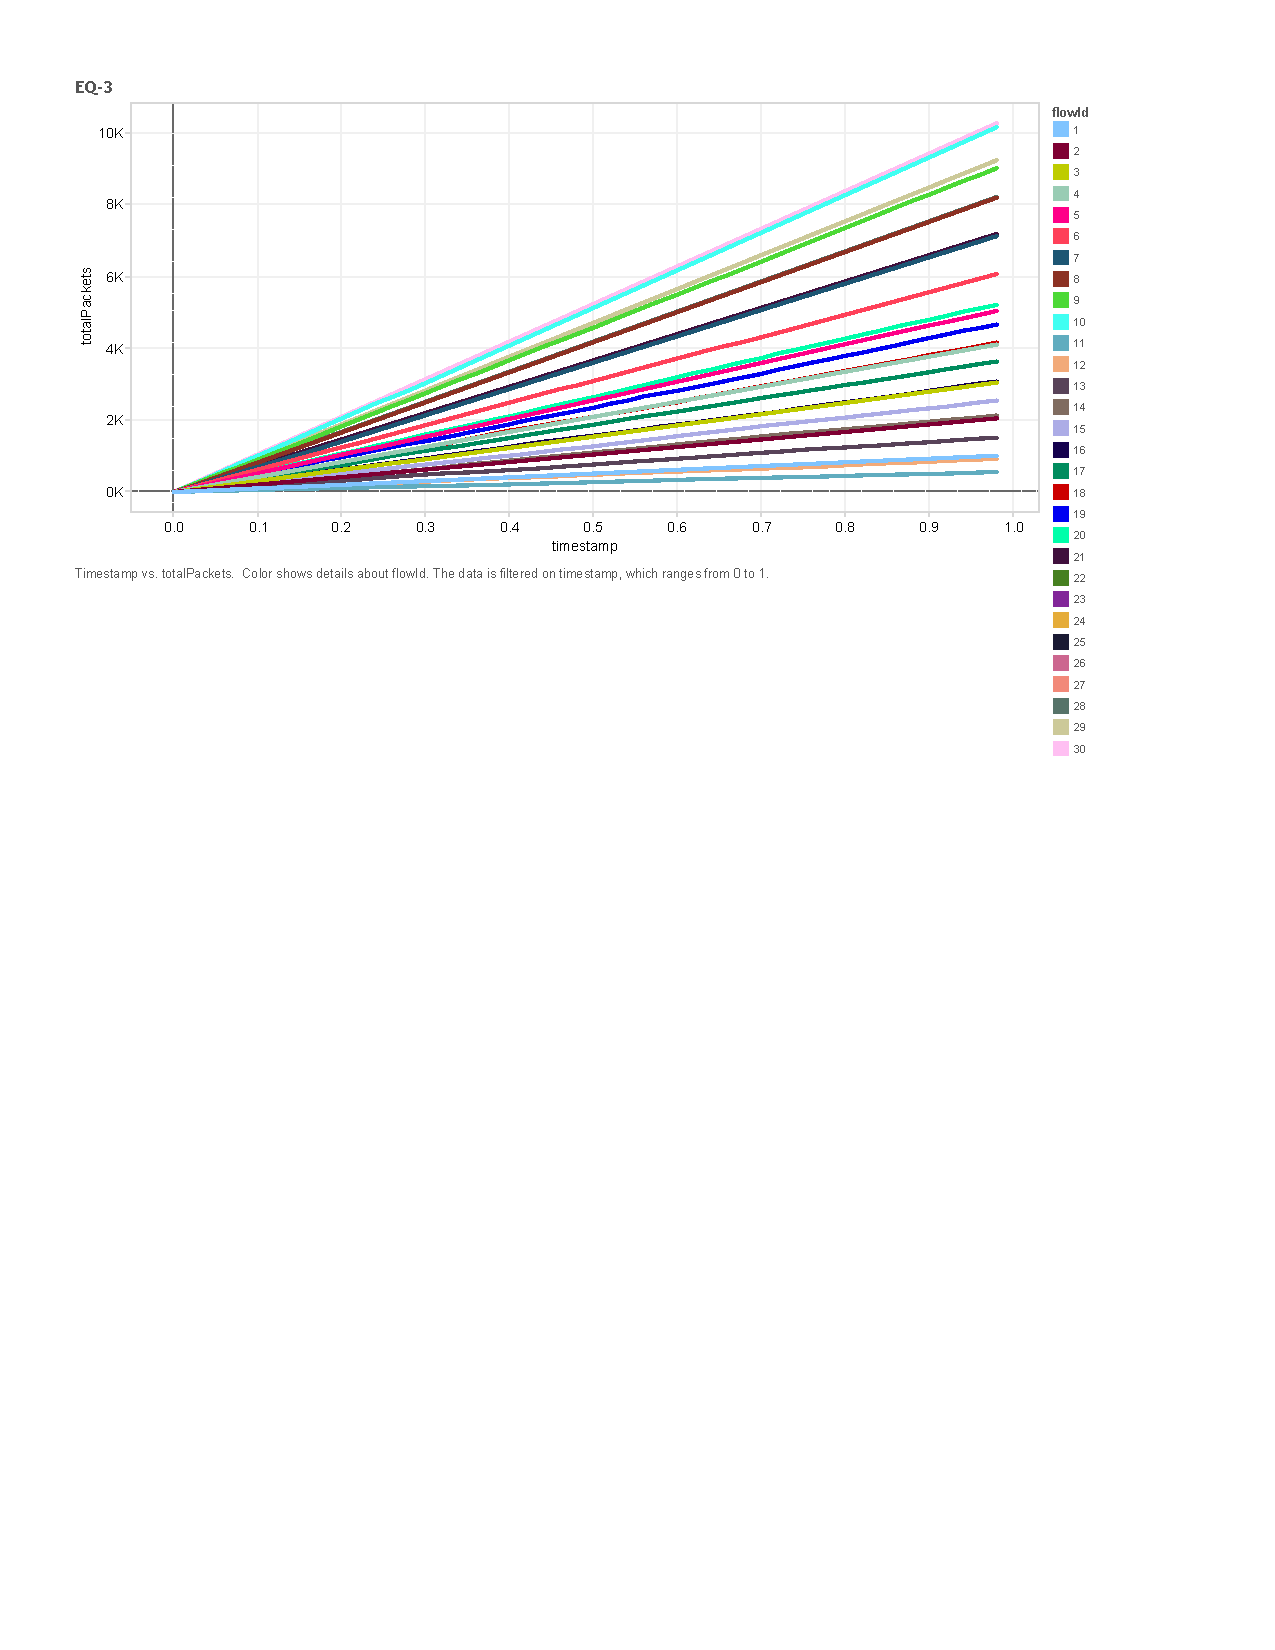
\includegraphics{plots/PEQ-EQ/EQ-3}

\caption{UU, Poisson, EQ \label{fig:UU,-Poisson,-EQ}}
\end{figure}


\pagebreak{}

Figure \ref{fig:UU,-Poisson,-PEQ} shows the behavior of PEQ scheduler.
As in the case of $EQ$, $C_{1}$ through $C_{10}$ are greedy and
always have non-empty queues, each of the group $C$ flows get a bandwidth
of nearly $11\; Mbytes/sec.$ on average and thus converge together
at a point above the plot of flow $A_{10}$. The plot is nearly identical
to that of $EQ$ scheduler.

\begin{figure}[H]
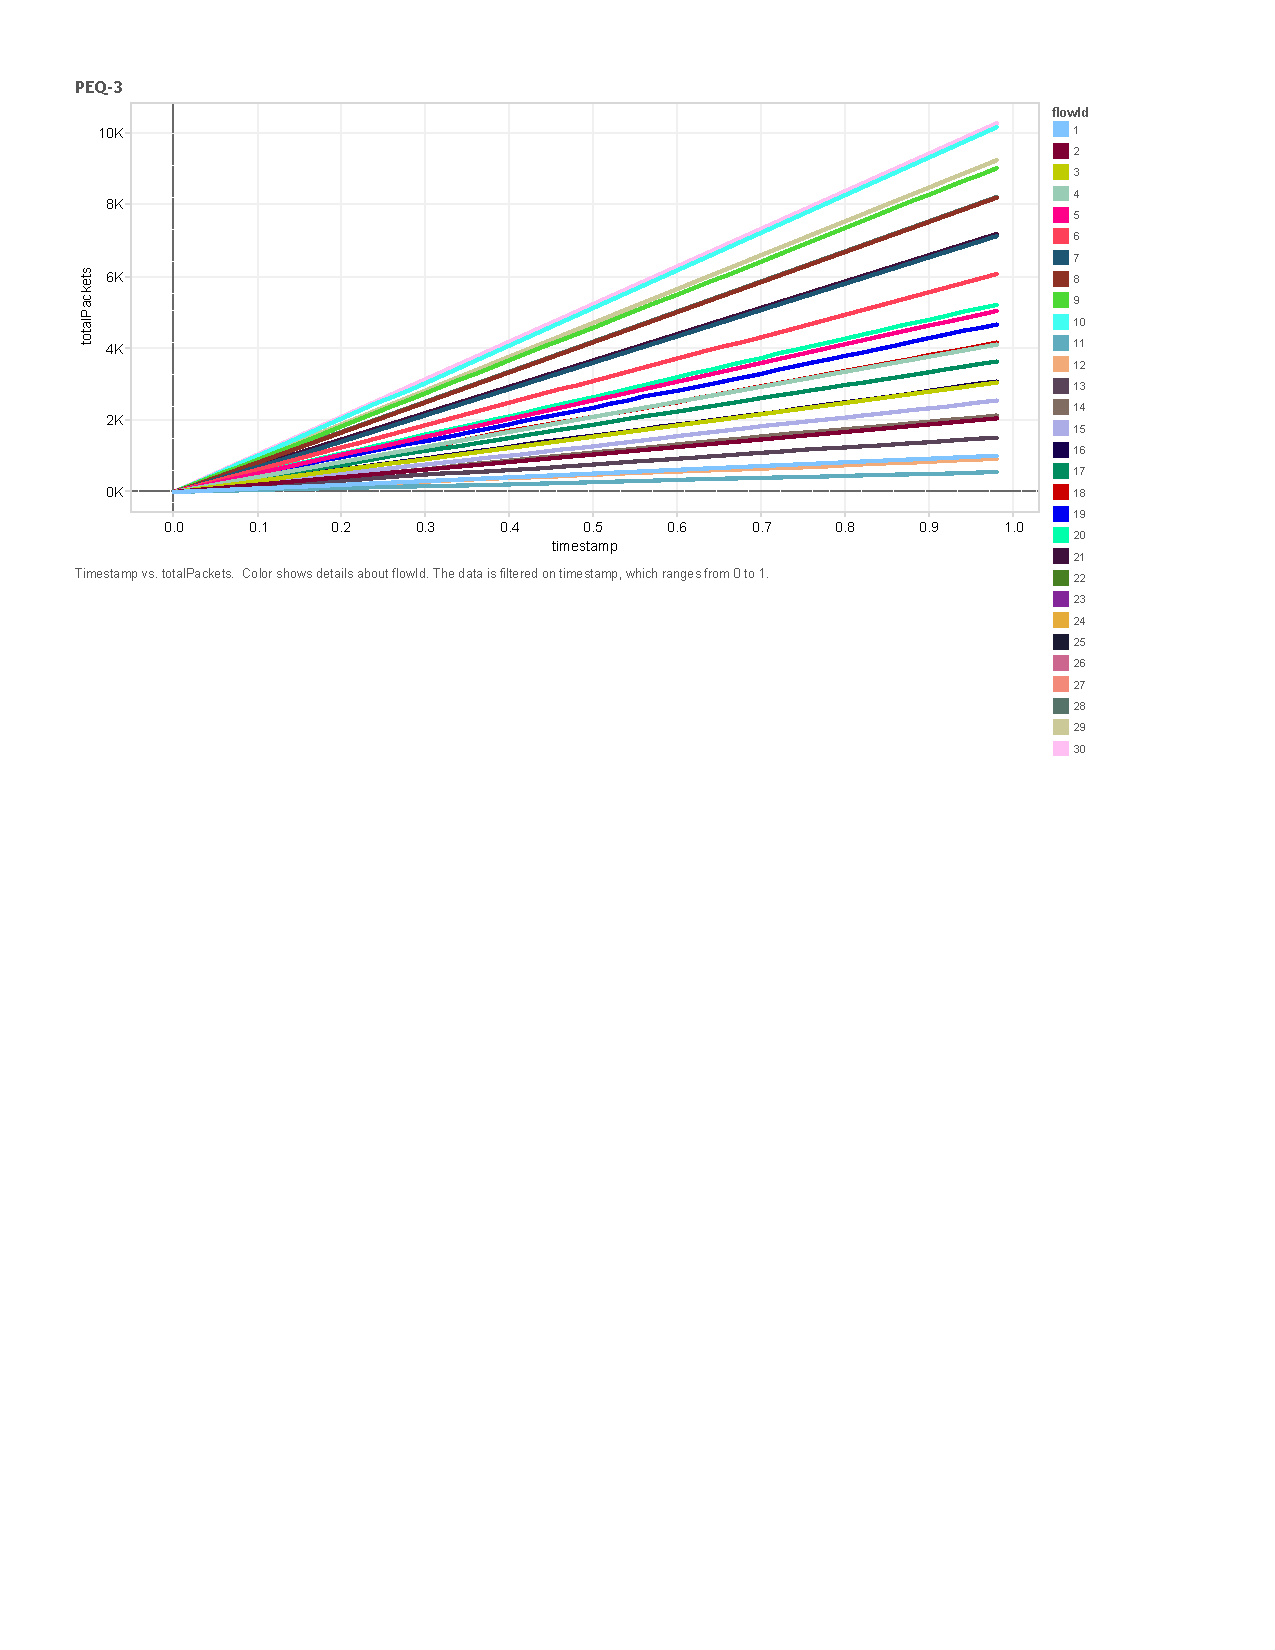
\includegraphics{plots/PEQ-EQ/PEQ-3}

\caption{UU, Poisson, PEQ \label{fig:UU,-Poisson,-PEQ} }
\end{figure}


\pagebreak{}

Figure \ref{fig:UU,-Poisson,-A-PEQ} shows the behavior of PEQ scheduler.
As in the case of $EQ$, $C_{1}$ through $C_{10}$ are greedy and
always have non-empty queues, each of the group $C$ flows get a bandwidth
of nearly $11\; Mbytes/sec.$ on average and thus converge together
at a point above the plot of flow $A_{10}$. The plot is nearly identical
to that of $EQ$ scheduler.

\begin{figure}[H]
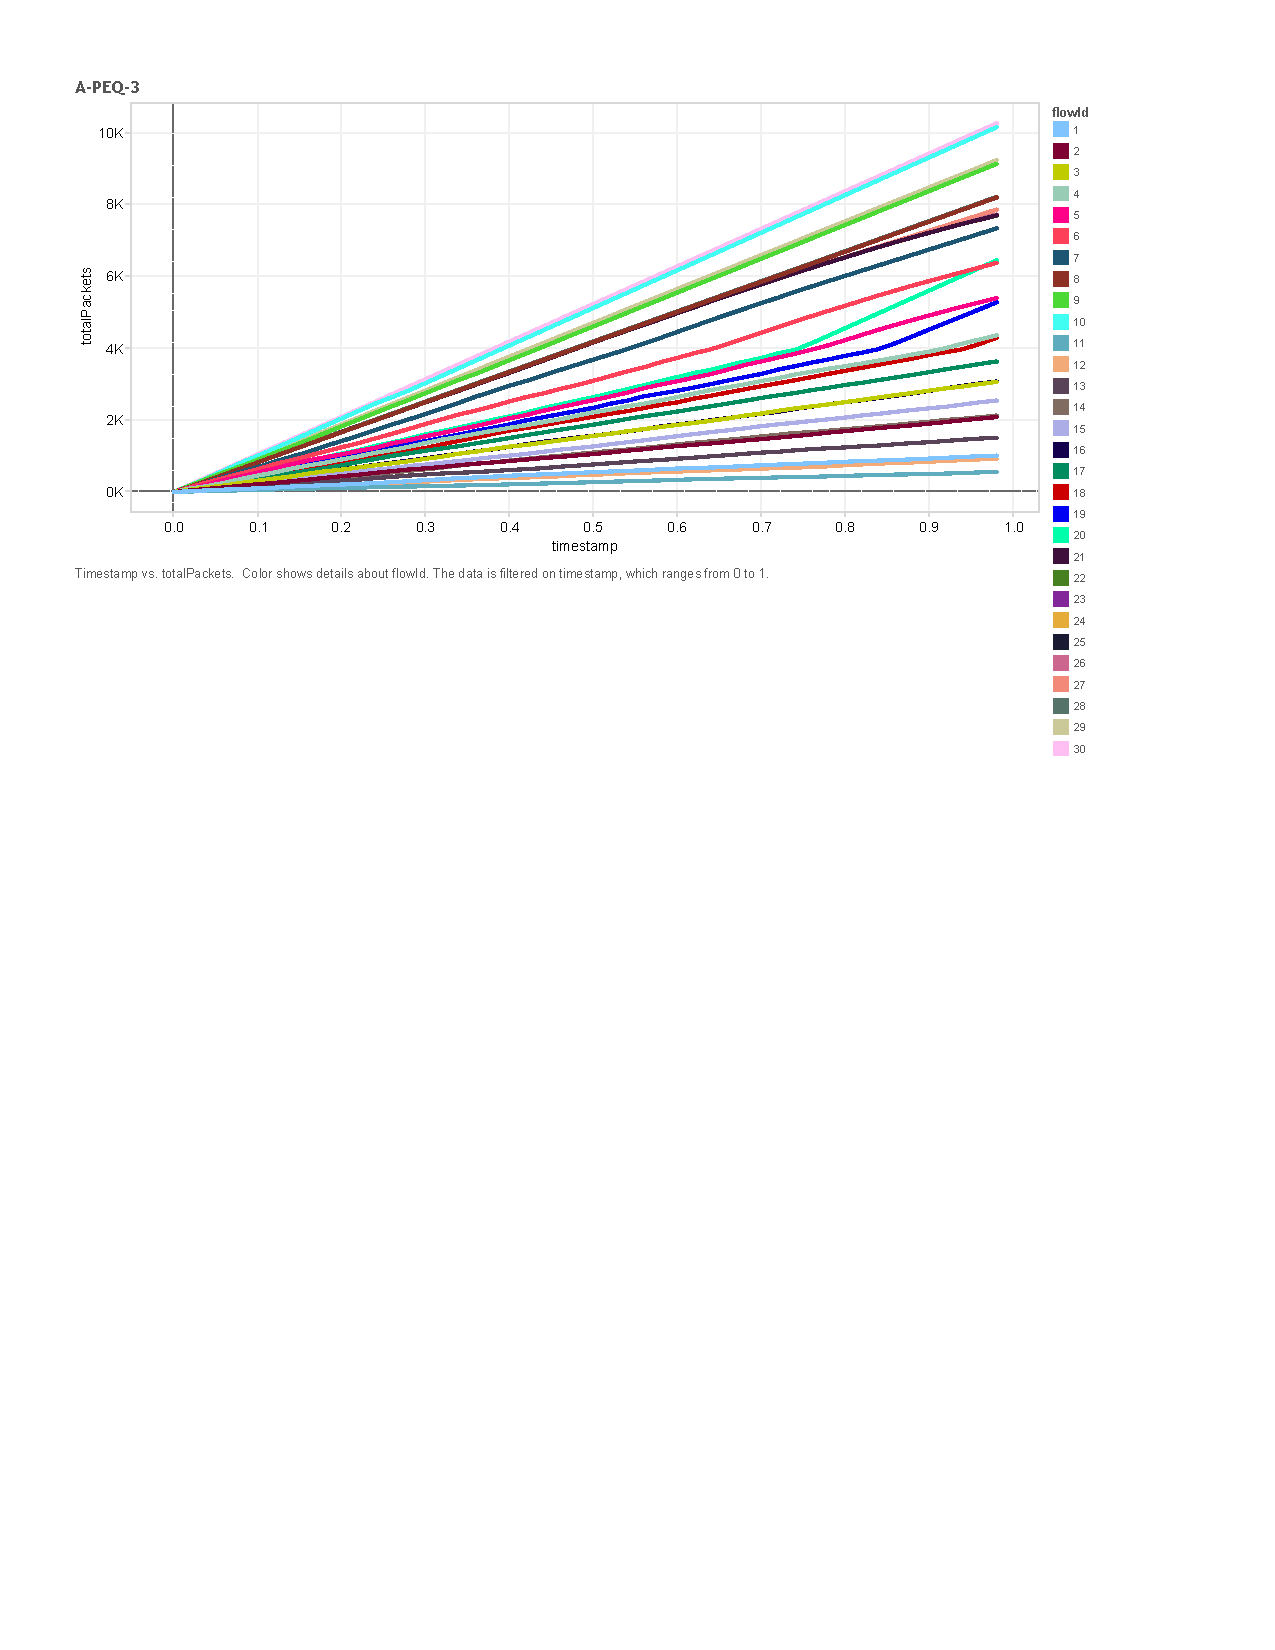
\includegraphics{plots/A-PEQ/A-PEQ-3}

\caption{UU, Poisson, A-PEQ \label{fig:UU,-Poisson,-A-PEQ} }
\end{figure}



\subsection{UU, Constant Rate}

In this scenario, two groups $A$ and $C$ are considered and flows
in group $A$ have a poisson arrival process. In the plots, flows
with id $1,\;2,\;....,\;10$ correspond to flows $A_{1}$ through
$A_{10}$ and flows with id $11,\;12,\;....,\;20$ correspond to flows
$C_{1}$ through $C_{10}$.

\vspace{40pt}

\begin{figure}[H]
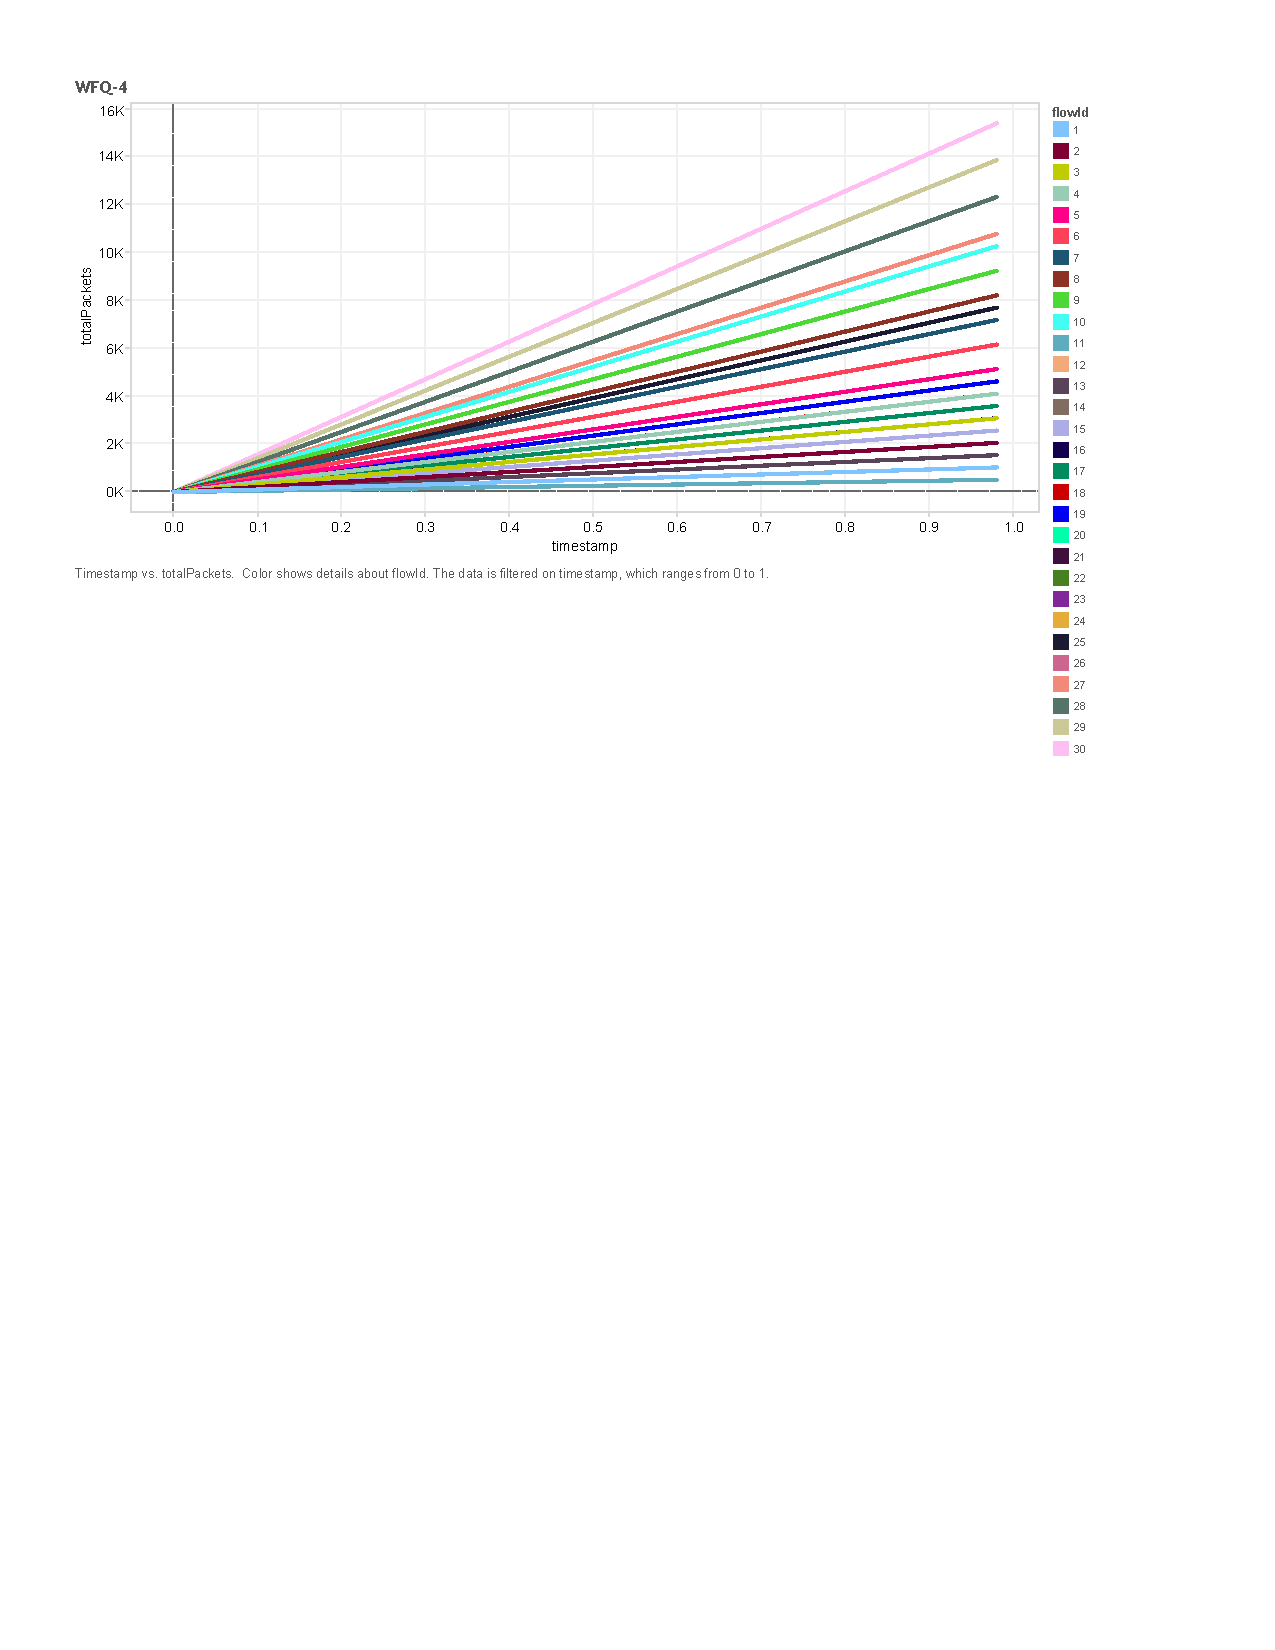
\includegraphics{plots/WFQ/WFQ-4}

\caption{UU, CR, WFQ\label{fig:UU,-CR,-WFQ}}
\end{figure}


Figure \ref{fig:UU,-CR,-WFQ} shows the behavior of $WFQ$. Since
flows $A_{1}$ through $A_{10}$ produce the packets at an average
rate equal to their reserved rates, they are not able to utilize the
extra bandwidth. However, since $C_{1}$ through $C_{10}$ are greedy
and always have non-empty queues, all of them get nearly twice the
bandwidth of the corresponding flows in group $A$, e.g. $C_{20}$
is able to transmit twice the number of packets than $A_{10}$ even
though both of them have a reserved rate of $10\; Mbytes/sec.$.

\pagebreak{}

Figure \ref{fig:UU,-CR,-EQ} shows the behavior of pure EQ scheduler.
Since flows $A_{1}$ through $A_{10}$ produce the packets at an average
rate equal to their reserved rates, they are not able to utilize the
extra bandwidth. However, since $C_{1}$ through $C_{10}$ are greedy
and always have non-empty queues, each of the group $C$ flows get
a bandwidth of nearly $11\; Mbytes/sec.$ and thus converge together
at a point above the plot of flow $A_{10}$.

\begin{figure}[H]
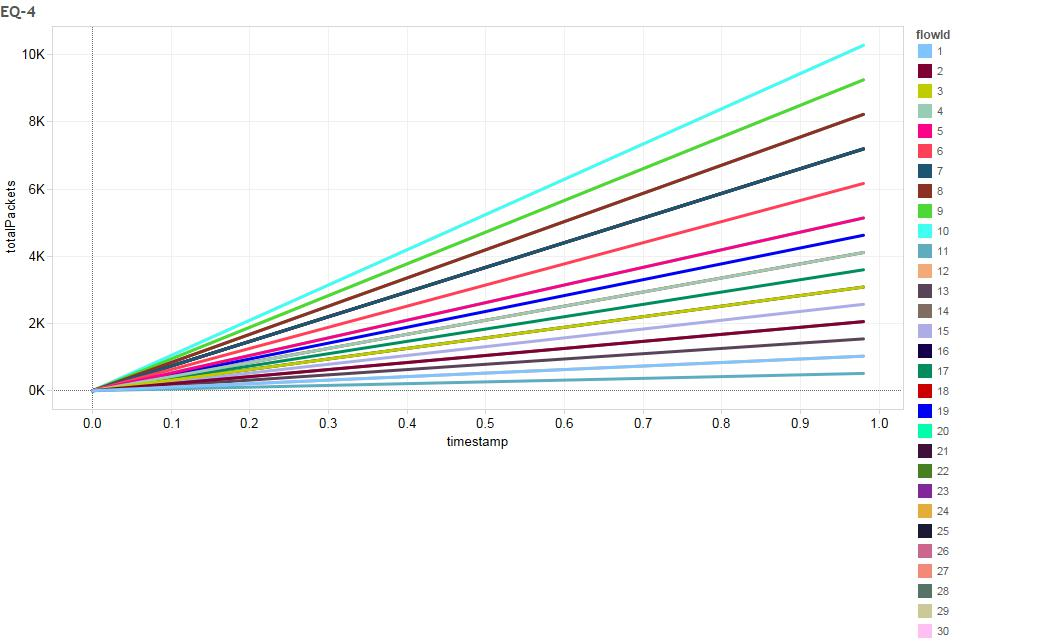
\includegraphics{plots/PEQ-EQ/EQ-4}

\caption{UU, CR, EQ \label{fig:UU,-CR,-EQ}}
\end{figure}


\pagebreak{}

Figure \ref{fig:UU,-CR,-PEQ} shows the behavior of PEQ scheduler.
As in the case of $EQ$, $C_{1}$ through $C_{10}$ are greedy and
always have non-empty queues, each of the group $C$ flows get a bandwidth
of nearly $11\; Mbytes/sec.$ on average and thus converge together
at a point above the plot of flow $A_{10}$. The plot is nearly identical
to that of $EQ$ scheduler.

\begin{figure}[H]
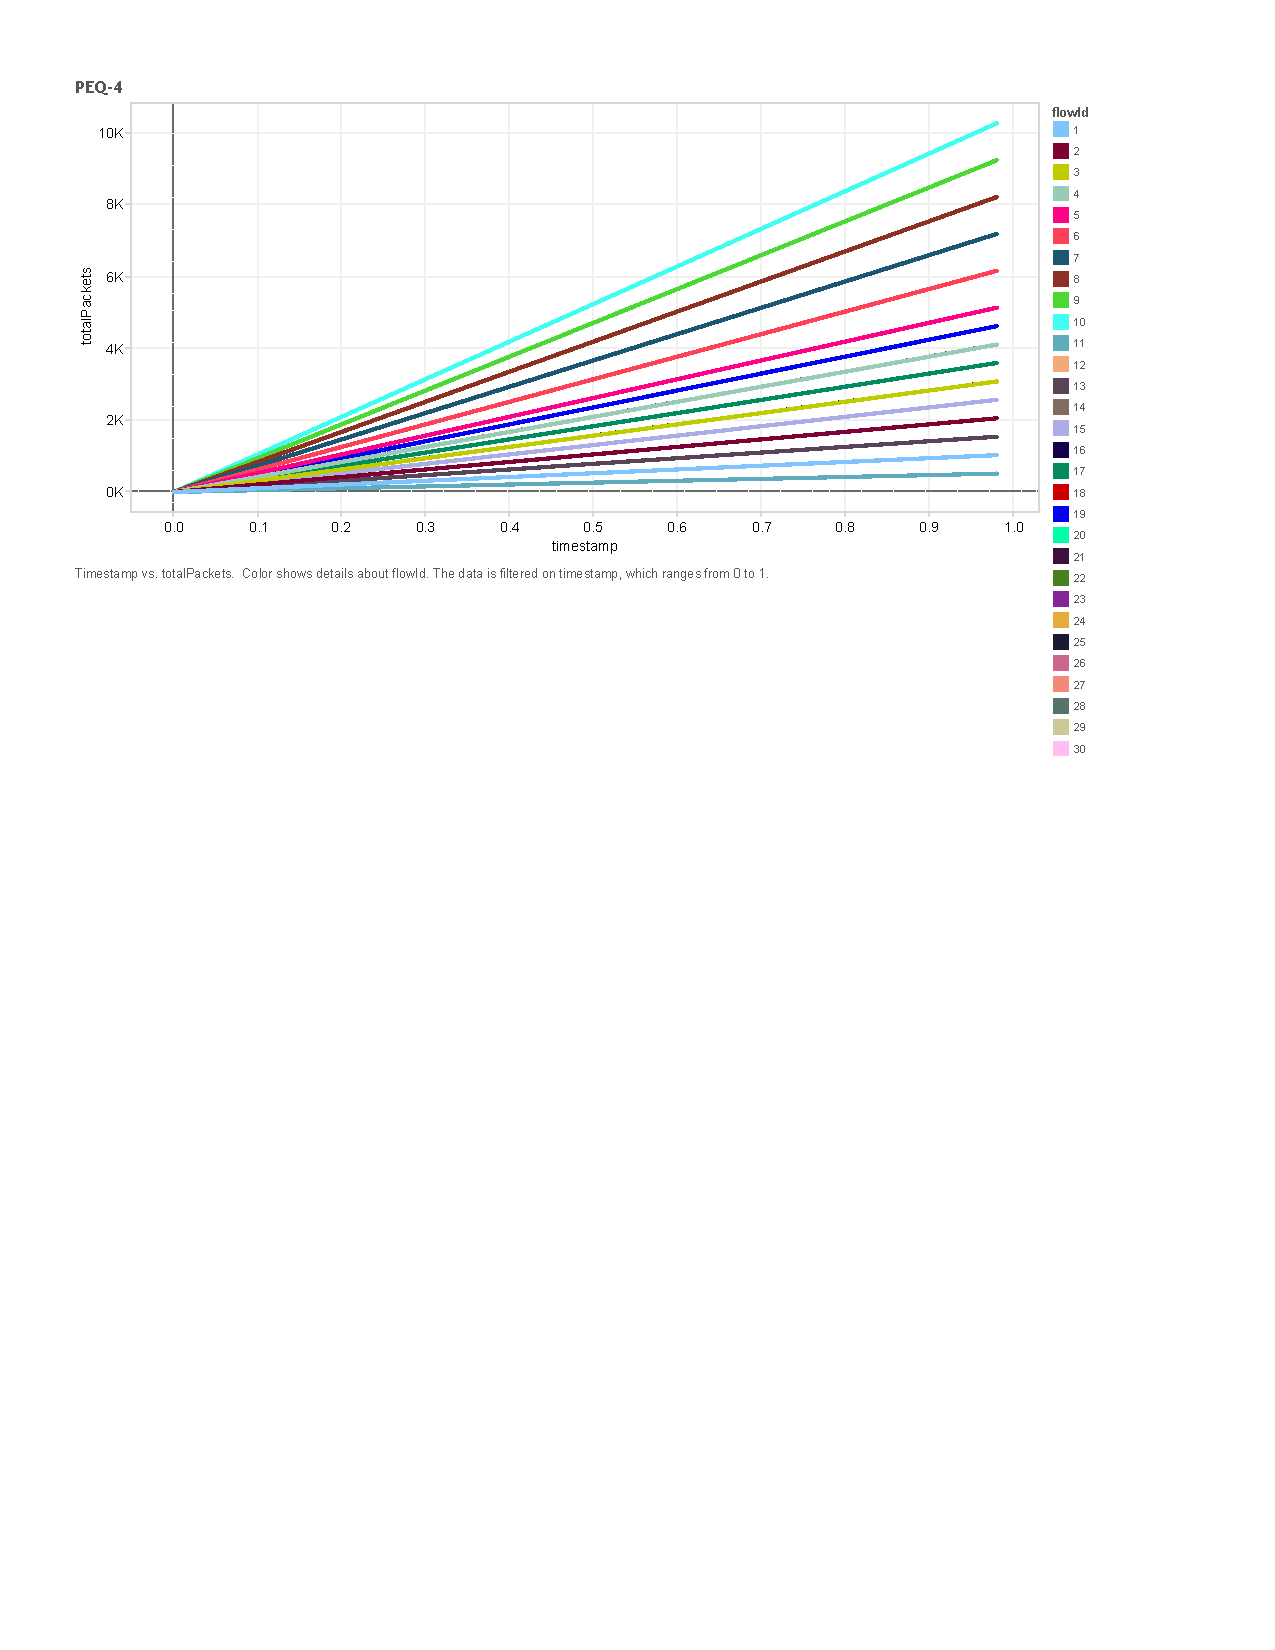
\includegraphics{plots/PEQ-EQ/PEQ-4}

\caption{UU, CR, PEQ \label{fig:UU,-CR,-PEQ} }
\end{figure}


\pagebreak{}

Figure \ref{fig:UU,-CR,-A-PEQ} shows the behavior of PEQ scheduler.
As in the case of $EQ$, $C_{1}$ through $C_{10}$ are greedy and
always have non-empty queues, each of the group $C$ flows get a bandwidth
of nearly $11\; Mbytes/sec.$ on average and thus converge together
at a point above the plot of flow $A_{10}$. The plot is nearly identical
to that of $EQ$ scheduler.

\begin{figure}[H]
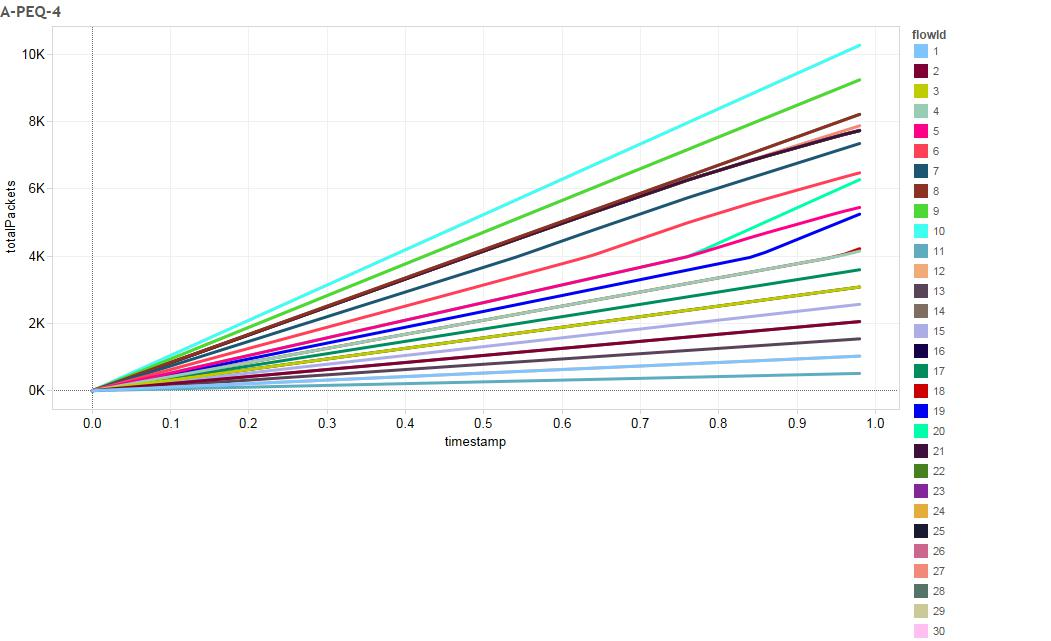
\includegraphics{plots/A-PEQ/A-PEQ-4}

\caption{UU, CR, A-PEQ \label{fig:UU,-CR,-A-PEQ} }
\end{figure}


\pagebreak{}


\subsection{UA + UU, Poisson}

In this scenario, two groups $A$ and $C$ are considered and flows
in group $A$ have a poisson arrival process. In the plots, flows
with id $1,\;2,\;....,\;10$ correspond to flows $A_{1}$ through
$A_{10}$ and flows with id $11,\;12,\;....,\;20$ correspond to flows
$C_{1}$ through $C_{10}$.

\vspace{40pt}

\begin{figure}[H]
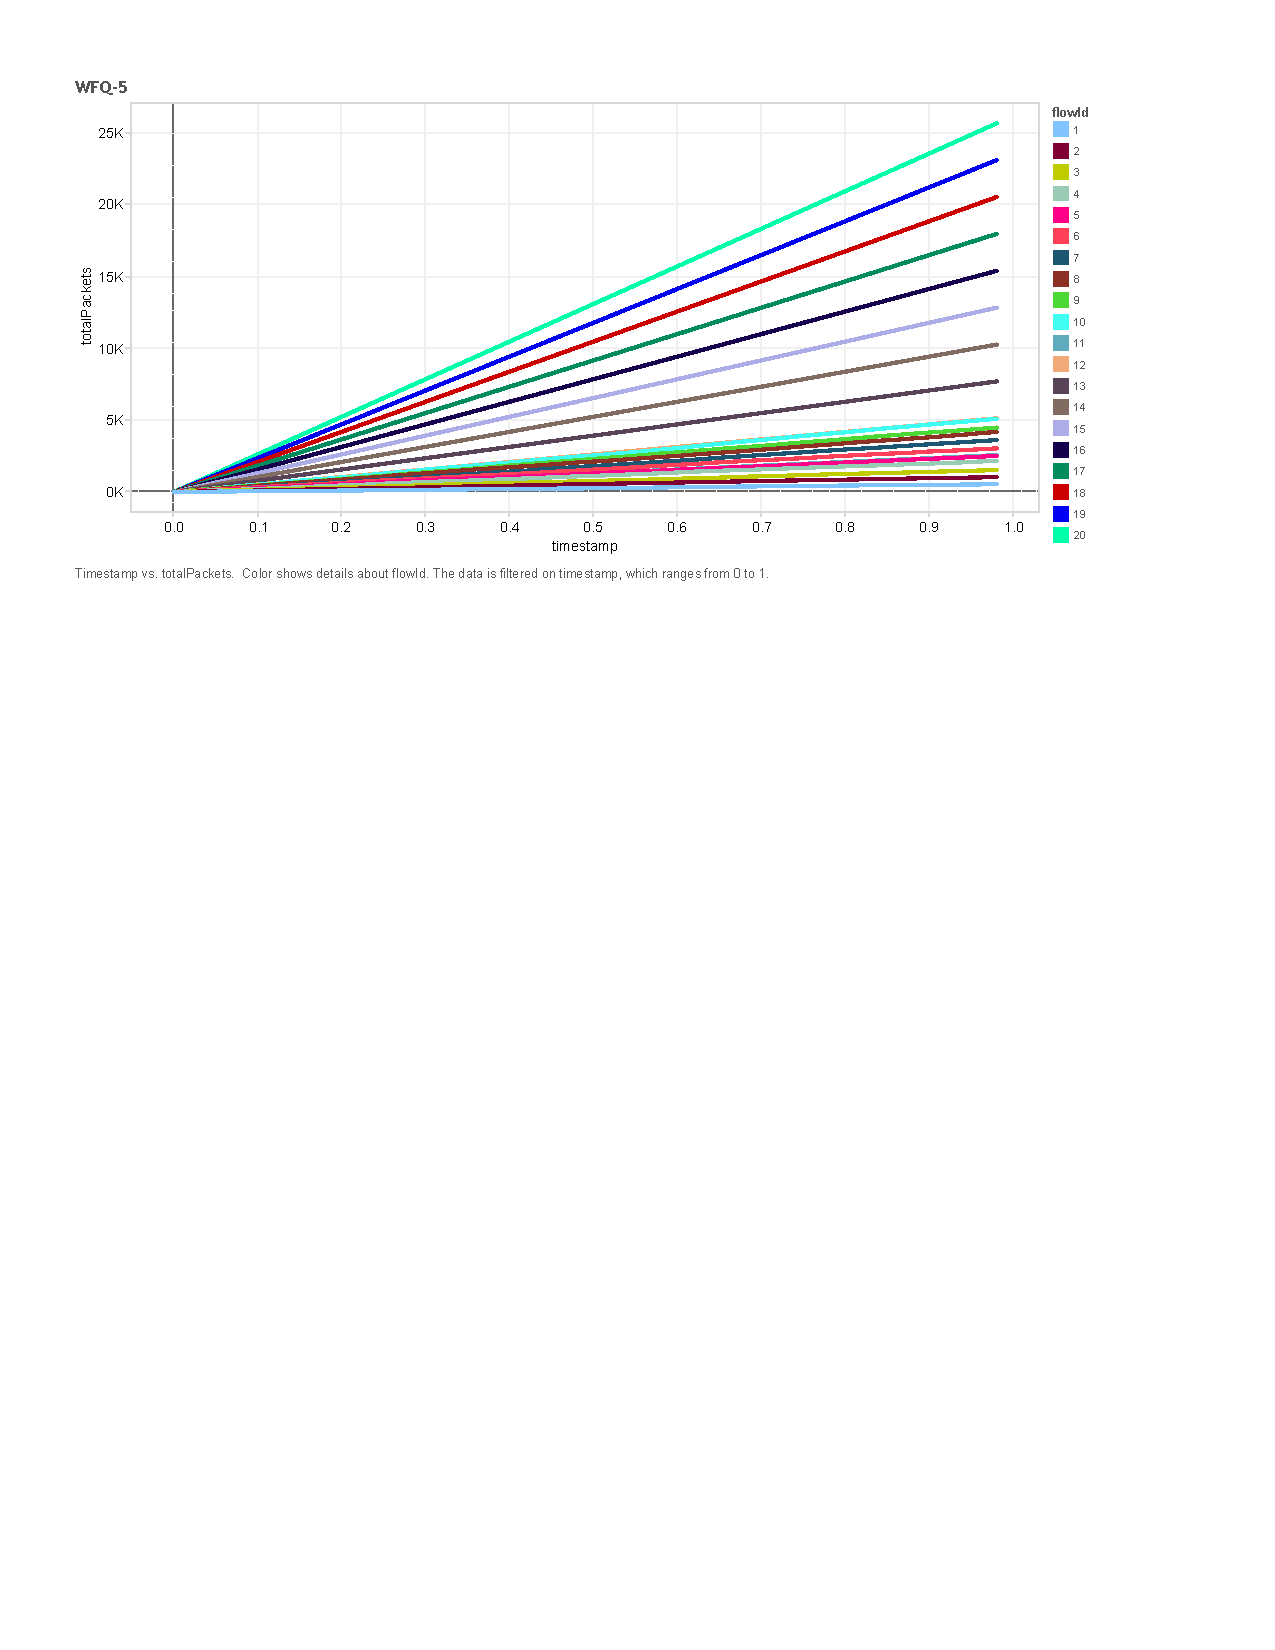
\includegraphics{plots/WFQ/WFQ-5}

\caption{UA + UU, Poisson, WFQ\label{fig:UA + UU,-Poisson,-WFQ}}
\end{figure}


Figure \ref{fig:UA + UU,-Poisson,-WFQ} shows the behavior of $WFQ$.
Since flows $A_{1}$ through $A_{10}$ produce the packets at an average
rate equal to their reserved rates, they are not able to utilize the
extra bandwidth. However, since $C_{1}$ through $C_{10}$ are greedy
and always have non-empty queues, all of them get nearly twice the
bandwidth of the corresponding flows in group $A$, e.g. $C_{20}$
is able to transmit twice the number of packets than $A_{10}$ even
though both of them have a reserved rate of $10\; Mbytes/sec.$.

\pagebreak{}

Figure \ref{fig:UA + UU,-Poisson,-EQ} shows the behavior of pure
EQ scheduler. Since flows $A_{1}$ through $A_{10}$ produce the packets
at an average rate equal to their reserved rates, they are not able
to utilize the extra bandwidth. However, since $C_{1}$ through $C_{10}$
are greedy and always have non-empty queues, each of the group $C$
flows get a bandwidth of nearly $11\; Mbytes/sec.$ and thus converge
together at a point above the plot of flow $A_{10}$.

\begin{figure}[H]
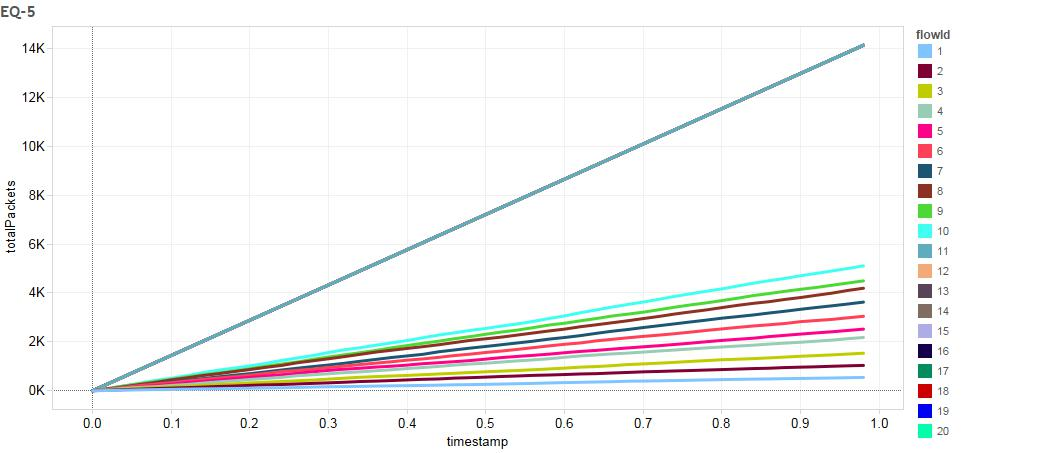
\includegraphics{plots/PEQ-EQ/EQ-5}

\caption{UA + UU, Poisson, EQ \label{fig:UA + UU,-Poisson,-EQ}}
\end{figure}


\pagebreak{}

Figure \ref{fig:UA + UA,-Poisson,-PEQ} shows the behavior of PEQ
scheduler. As in the case of $EQ$, $C_{1}$ through $C_{10}$ are
greedy and always have non-empty queues, each of the group $C$ flows
get a bandwidth of nearly $11\; Mbytes/sec.$ on average and thus
converge together at a point above the plot of flow $A_{10}$. The
plot is nearly identical to that of $EQ$ scheduler.

\begin{figure}[H]
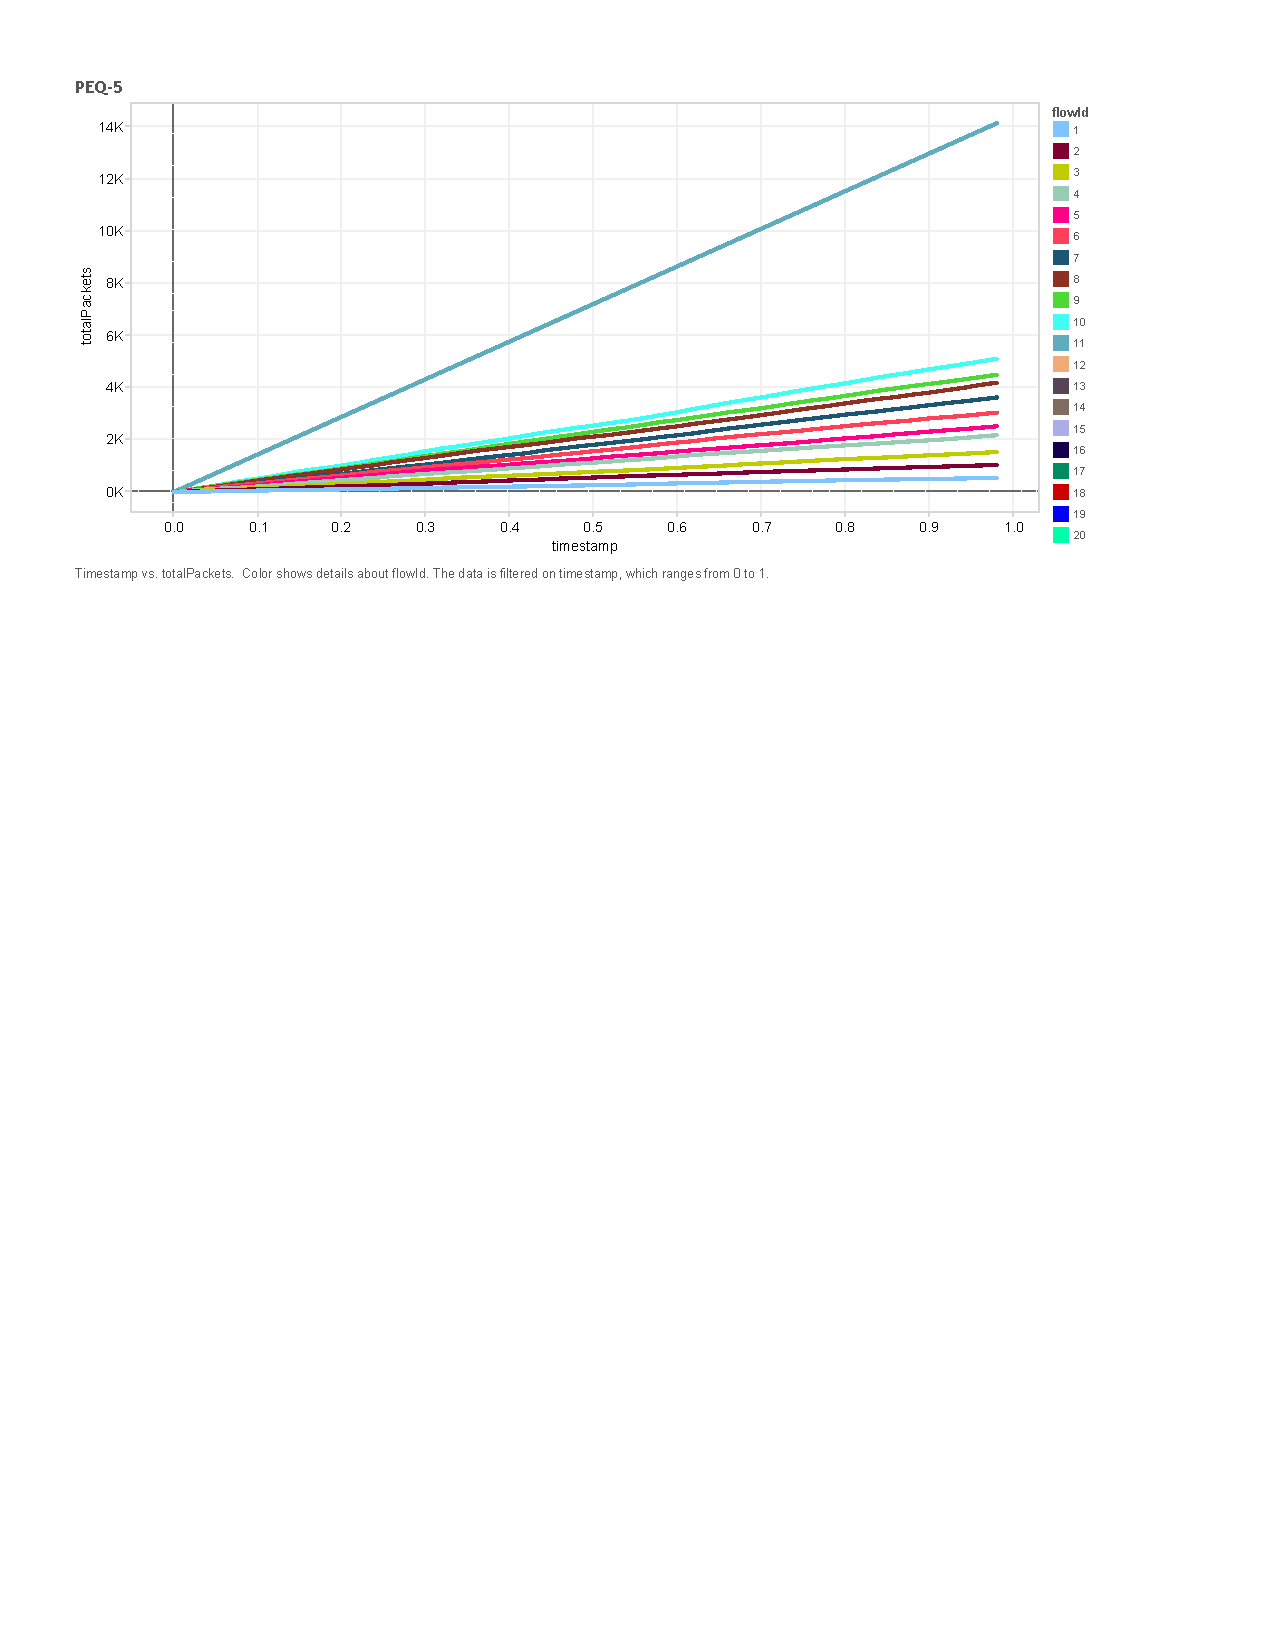
\includegraphics{plots/PEQ-EQ/PEQ-5}

\caption{UA + UU, Poisson, PEQ \label{fig:UA + UA,-Poisson,-PEQ} }
\end{figure}


\pagebreak{}

Figure \ref{fig:UA + UU,-Poisson,-A-PEQ} shows the behavior of PEQ
scheduler. As in the case of $EQ$, $C_{1}$ through $C_{10}$ are
greedy and always have non-empty queues, each of the group $C$ flows
get a bandwidth of nearly $11\; Mbytes/sec.$ on average and thus
converge together at a point above the plot of flow $A_{10}$. The
plot is nearly identical to that of $EQ$ scheduler.

\begin{figure}[H]
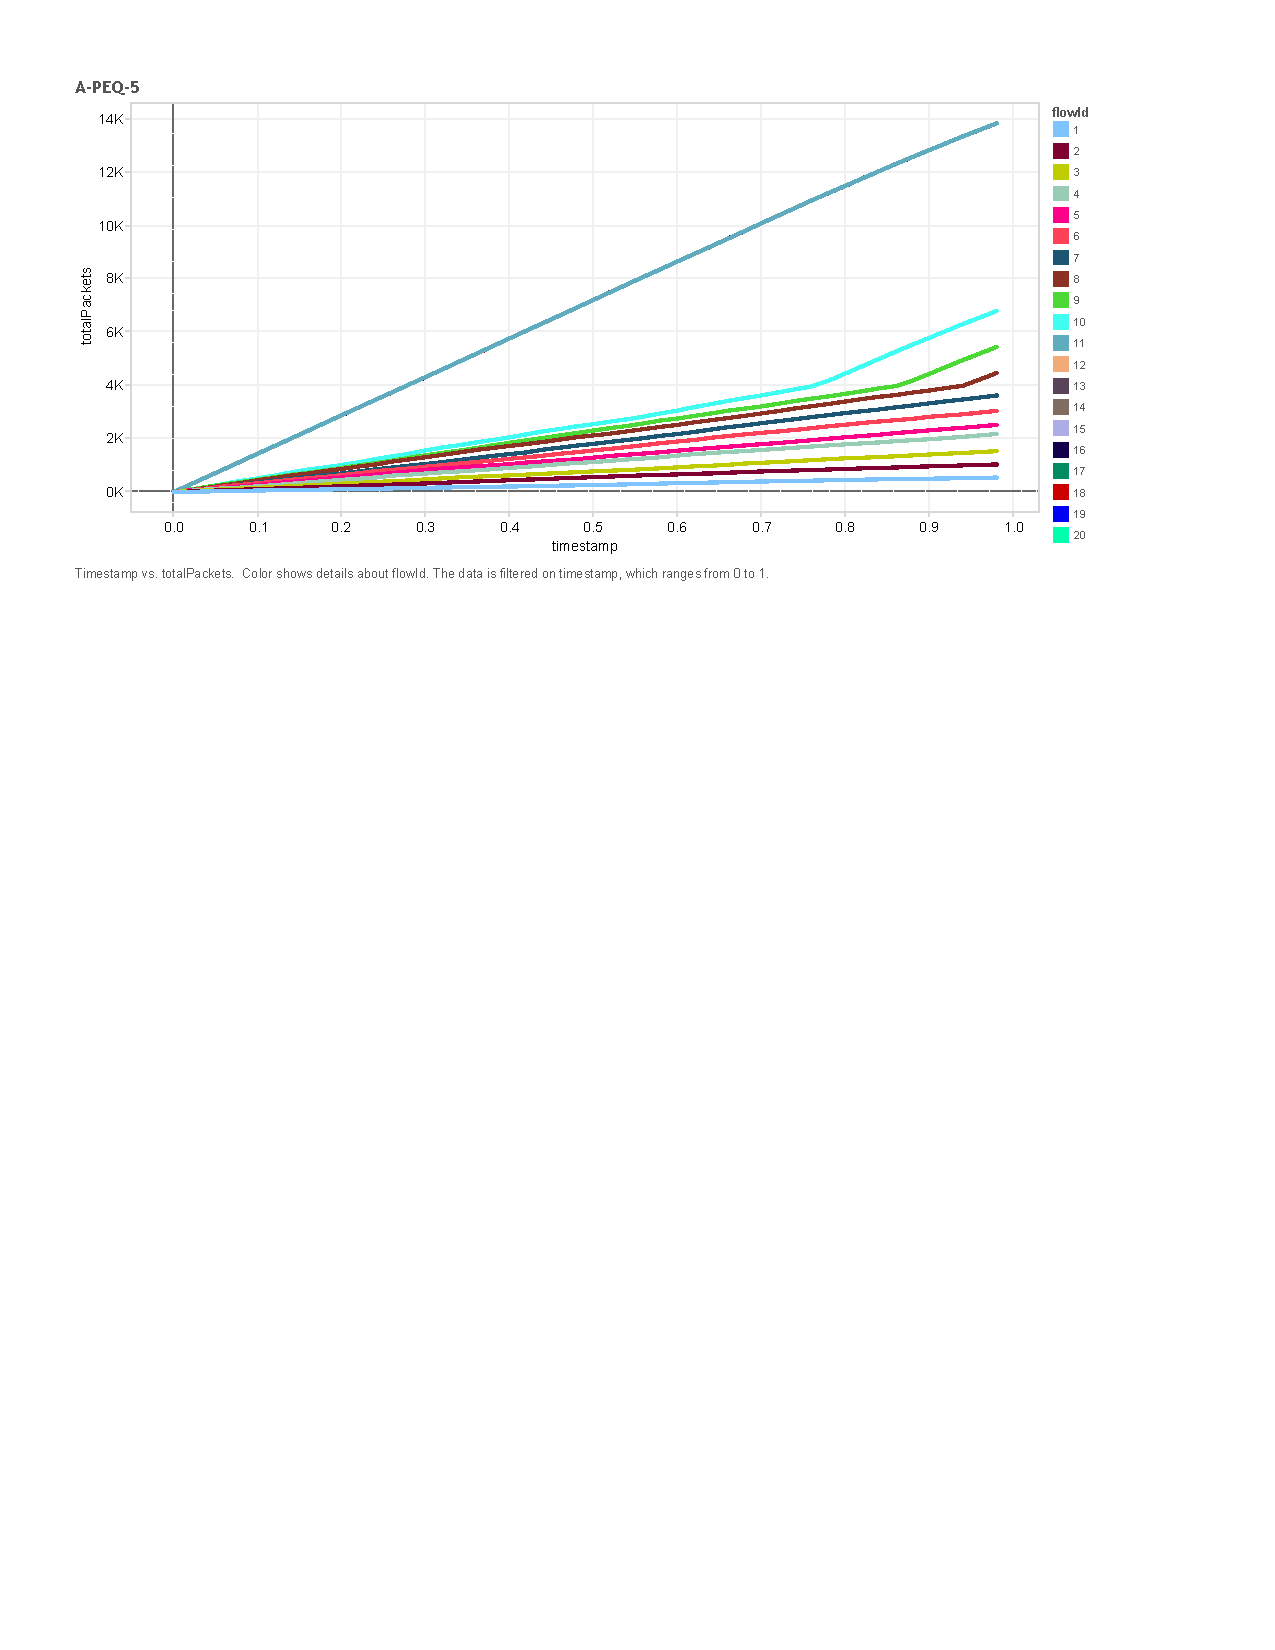
\includegraphics{plots/A-PEQ/A-PEQ-5}

\caption{UA + UU, Poisson, A-PEQ \label{fig:UA + UU,-Poisson,-A-PEQ} }
\end{figure}


\pagebreak{}


\subsection{UA + UU, Constant Rate}

In this scenario, two groups $A$ and $C$ are considered and flows
in group $A$ have a poisson arrival process. In the plots, flows
with id $1,\;2,\;....,\;10$ correspond to flows $A_{1}$ through
$A_{10}$ and flows with id $11,\;12,\;....,\;20$ correspond to flows
$C_{1}$ through $C_{10}$.

\vspace{40pt}

\begin{figure}[H]
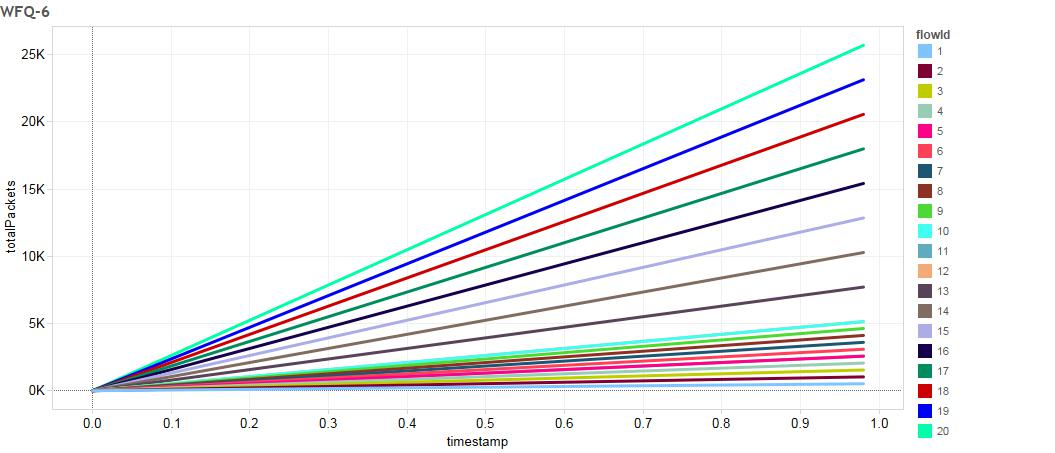
\includegraphics{plots/WFQ/WFQ-6}

\caption{UA + UU, CR, WFQ\label{fig:UA + UU,-CR,-WFQ}}
\end{figure}


Figure \ref{fig:UA + UU,-CR,-WFQ} shows the behavior of $WFQ$. Since
flows $A_{1}$ through $A_{10}$ produce the packets at an average
rate equal to their reserved rates, they are not able to utilize the
extra bandwidth. However, since $C_{1}$ through $C_{10}$ are greedy
and always have non-empty queues, all of them get nearly twice the
bandwidth of the corresponding flows in group $A$, e.g. $C_{20}$
is able to transmit twice the number of packets than $A_{10}$ even
though both of them have a reserved rate of $10\; Mbytes/sec.$.

\pagebreak{}

Figure \ref{fig:UA + UU,-CR,-EQ} shows the behavior of pure EQ scheduler.
Since flows $A_{1}$ through $A_{10}$ produce the packets at an average
rate equal to their reserved rates, they are not able to utilize the
extra bandwidth. However, since $C_{1}$ through $C_{10}$ are greedy
and always have non-empty queues, each of the group $C$ flows get
a bandwidth of nearly $11\; Mbytes/sec.$ and thus converge together
at a point above the plot of flow $A_{10}$.

\begin{figure}[H]
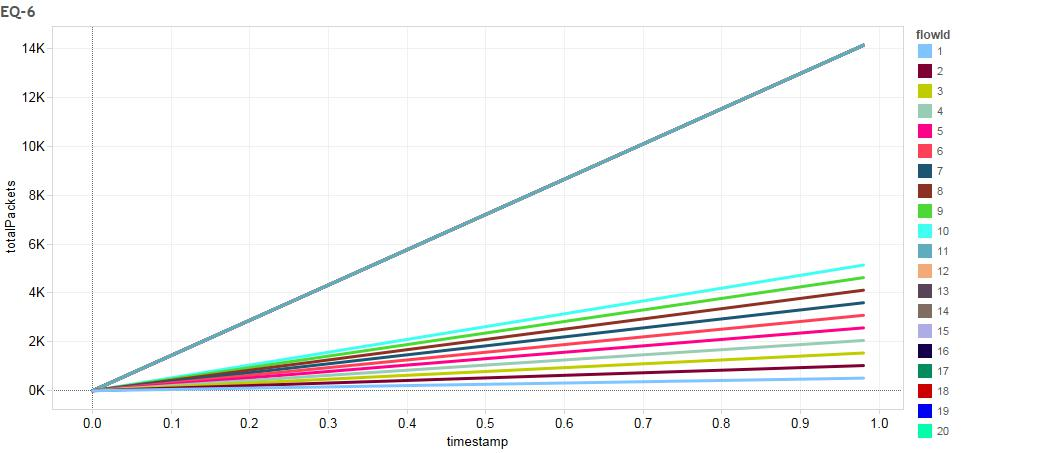
\includegraphics{plots/PEQ-EQ/EQ-6}

\caption{UA + UU, CR, EQ \label{fig:UA + UU,-CR,-EQ}}
\end{figure}


\pagebreak{}

Figure \ref{fig:UA + UA,-CR,-PEQ} shows the behavior of PEQ scheduler.
As in the case of $EQ$, $C_{1}$ through $C_{10}$ are greedy and
always have non-empty queues, each of the group $C$ flows get a bandwidth
of nearly $11\; Mbytes/sec.$ on average and thus converge together
at a point above the plot of flow $A_{10}$. The plot is nearly identical
to that of $EQ$ scheduler.

\begin{figure}[H]
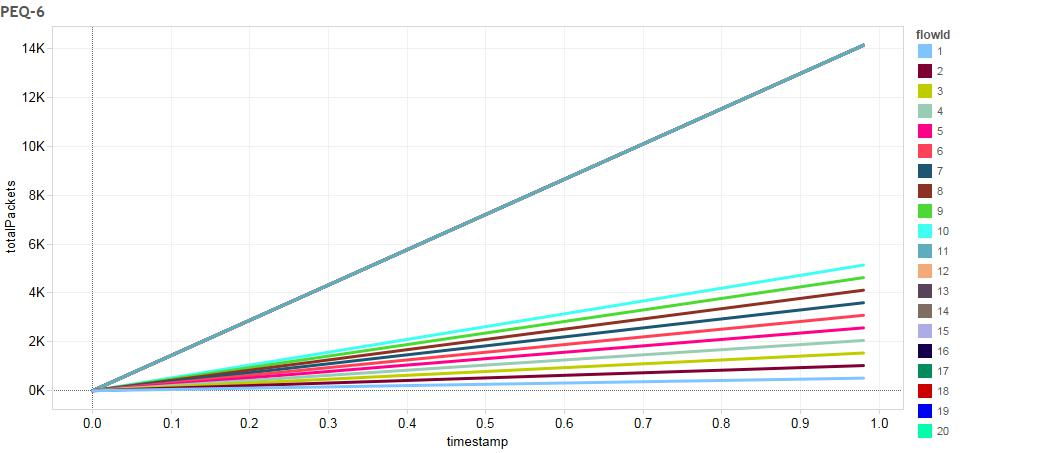
\includegraphics{plots/PEQ-EQ/PEQ-6}

\caption{UA + UU, CR, PEQ \label{fig:UA + UA,-CR,-PEQ} }
\end{figure}


\pagebreak{}

Figure \ref{fig:UA + UU,-CR,-A-PEQ} shows the behavior of PEQ scheduler.
As in the case of $EQ$, $C_{1}$ through $C_{10}$ are greedy and
always have non-empty queues, each of the group $C$ flows get a bandwidth
of nearly $11\; Mbytes/sec.$ on average and thus converge together
at a point above the plot of flow $A_{10}$. The plot is nearly identical
to that of $EQ$ scheduler.

\begin{figure}[H]
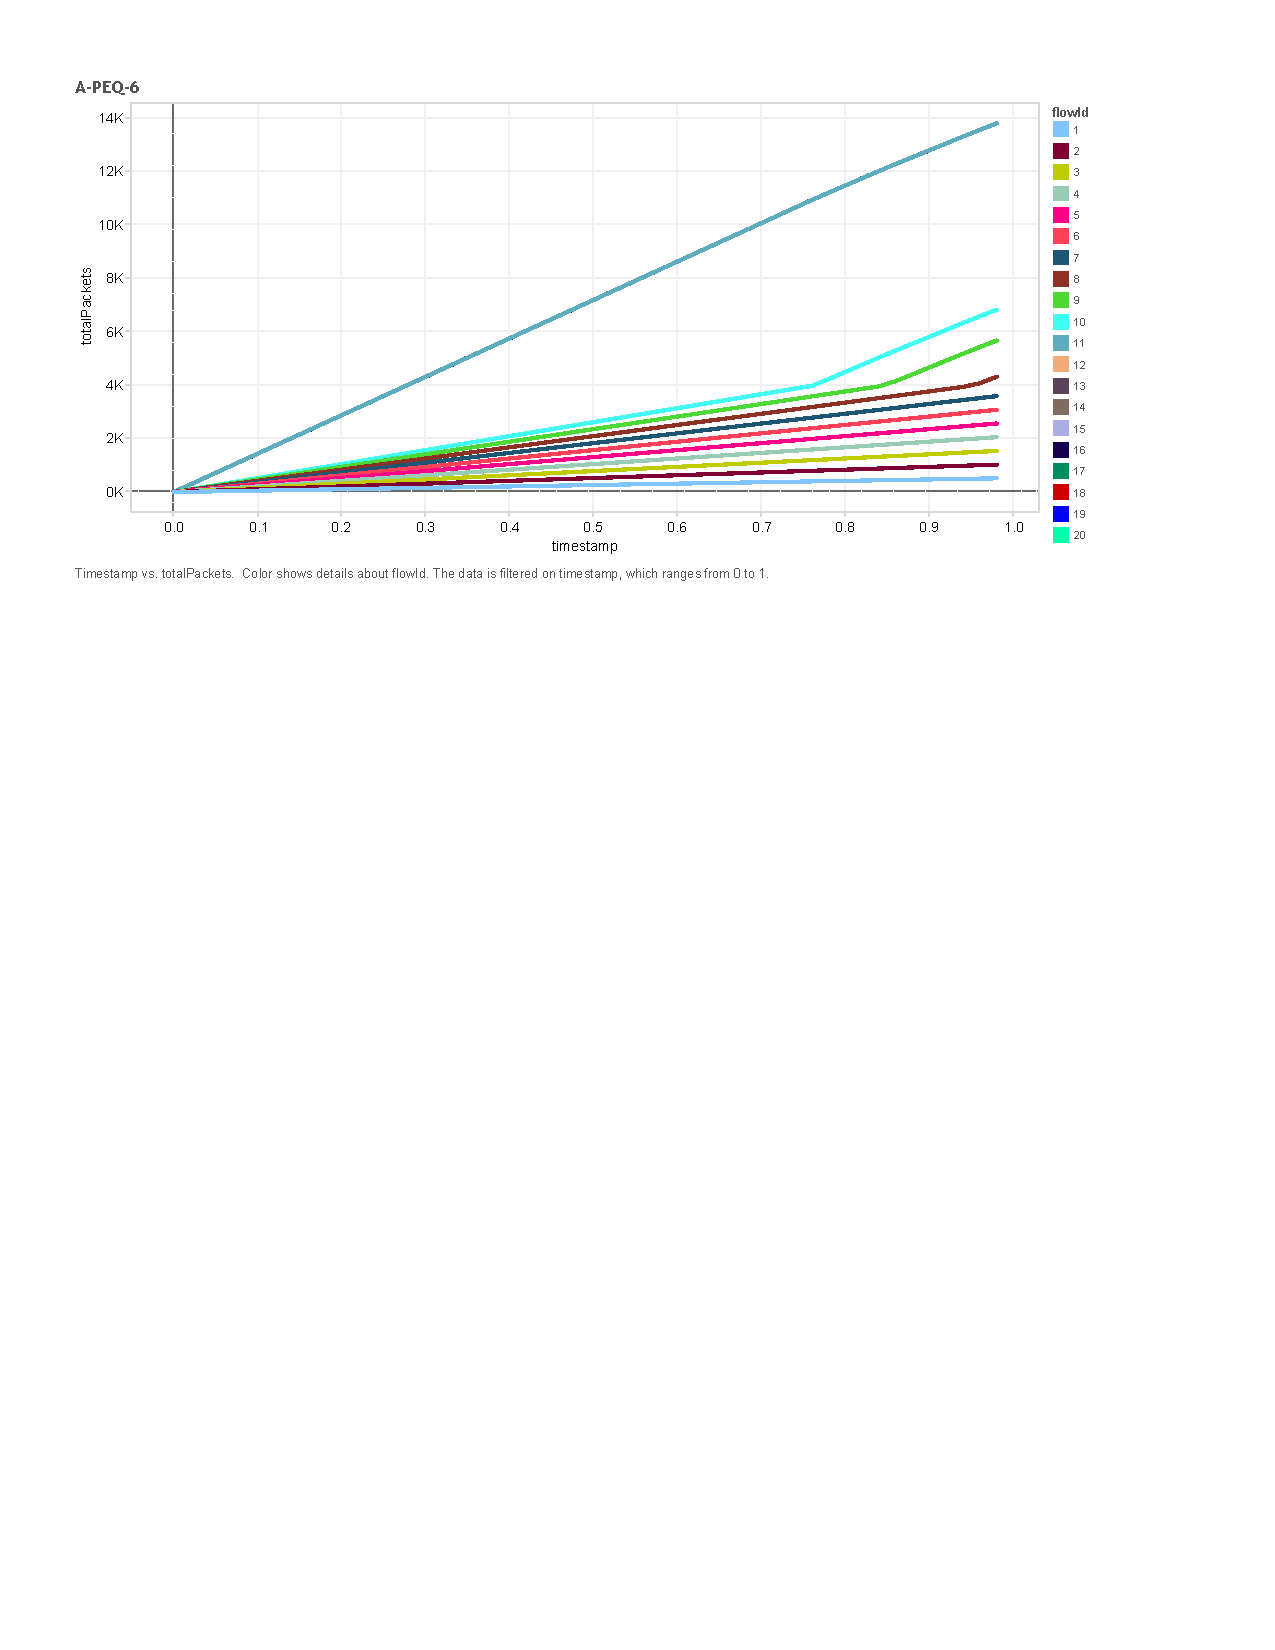
\includegraphics{plots/A-PEQ/A-PEQ-6}

\caption{UA + UU, CR, A-PEQ \label{fig:UA + UU,-CR,-A-PEQ} }
\end{figure}


\noindent \bibliographystyle{plainnat}
\bibliography{IEEEabrv,paper/bibliography}

\end{document}
